\chapter{Auswertung}
\label{auswertung}
Im Rahmen dieses Abschnitts werden die verschiedenen Phänomene und Aspekte, die bereits bei der Betrachtung und Interpretation der Ergebnisse der Messreihe angesprochen werden, nochmals aufgegriffen und isoliert betrachtet. Dabei werden hauptsächlich die Durchsatzergebnisse herangezogen, da der Fokus bei der Besprechung der Messreihen in \autoref{ergebnisse} bereits hauptsächlich auf die Latenzwerte gelegt wird. So werden auch die Durchsatzangaben nochmals genauer aufgegriffen. Außerdem wird in \autoref{ergebnisse} bereits die Beobachtung gemacht, dass Latenz- und Durchsatzwerte beide ähnliche Ergebnisse aufweisen. Ist bei einer Messung der Durchsatz hoch weist diese auch eine niedrige Latenz auf und umgekehrt.

\section{Einordnung der Performance}
\label{auswertung:einordnung}
Bei der Beurteilung der Performance der Datenbanksysteme handelt es sich bei den im Rahmen der Arbeit erzielten Messergebnissen um eine einfache Aufgabe. So weist bei jeder Messreihe Neo4j den niedrigsten Latenz- und Durchsatzwert auf, gefolgt von Db2 Graph Beta 3 -- sollte es Teil der Messreihe sein -- und Db2 Graph V11.5.6.0. 

Bei der Betrachtung der in der Messreihe beschriebenen Ergebnisse fällt zugleich auf, dass es sich hierbei nicht um einen kleinen Unterschied zwischen den jeweiligen Datenbanksystemen handelt. So scheinen sich die Datenbanksysteme sowohl bei der durchschnittlichen Latenz als auch beim Durchsatz um einen ähnlichen Faktor zu unterscheiden. Um die Datenbanksysteme bezüglich ihrer Performance einordnen zu können, wäre ein solcher Performance-Faktor ein passendes Maß. 

Um eine dementsprechende Kennzahl zur Einordnung der Datenbanksysteme bezüglich ihrer Performance bereitstellen zu können, wird daher ein gemeinsamer Durchschnittswert für den Durchsatz der Operationen:
\begin{itemize}
    \item \texttt{getNode}
    \item \texttt{getLink}
    \item \texttt{countLink} und 
    \item \texttt{getLinkList} (Range-Limit 100) ermittelt.
\end{itemize}
Der gemeinsame Durchschnittswert für den Durchsatz wird dabei einmal für jedes Datenbanksystem im Kontext einer Messreihe ermittelt. Anschließend wird der niedrigste Wert einer Messreihe herangezogen -- immer Db2 Graph V11.5.6.0 -- und als Faktor eins festgelegt. Im nächsten Schritt werden basierend auf diesem Faktor eins und seinem Durchschnittswert die jeweiligen Faktoren für Neo4j und gegebenenfalls Db2 Graph Beta 3 errechnet. Die dabei erhaltenen Performance-Faktoren -- basierend auf dem Durchsatz -- werden für die Messreihen mit einem konstant-verteilten Datensatz in \autoref{fig:faktor:durchsatz:const} dargelegt, während die mit real-verteilten Datensätzen in \autoref{fig:faktor:durchsatz:real} abgebildet werden.

\begin{figure}[!ht]
    \centering
    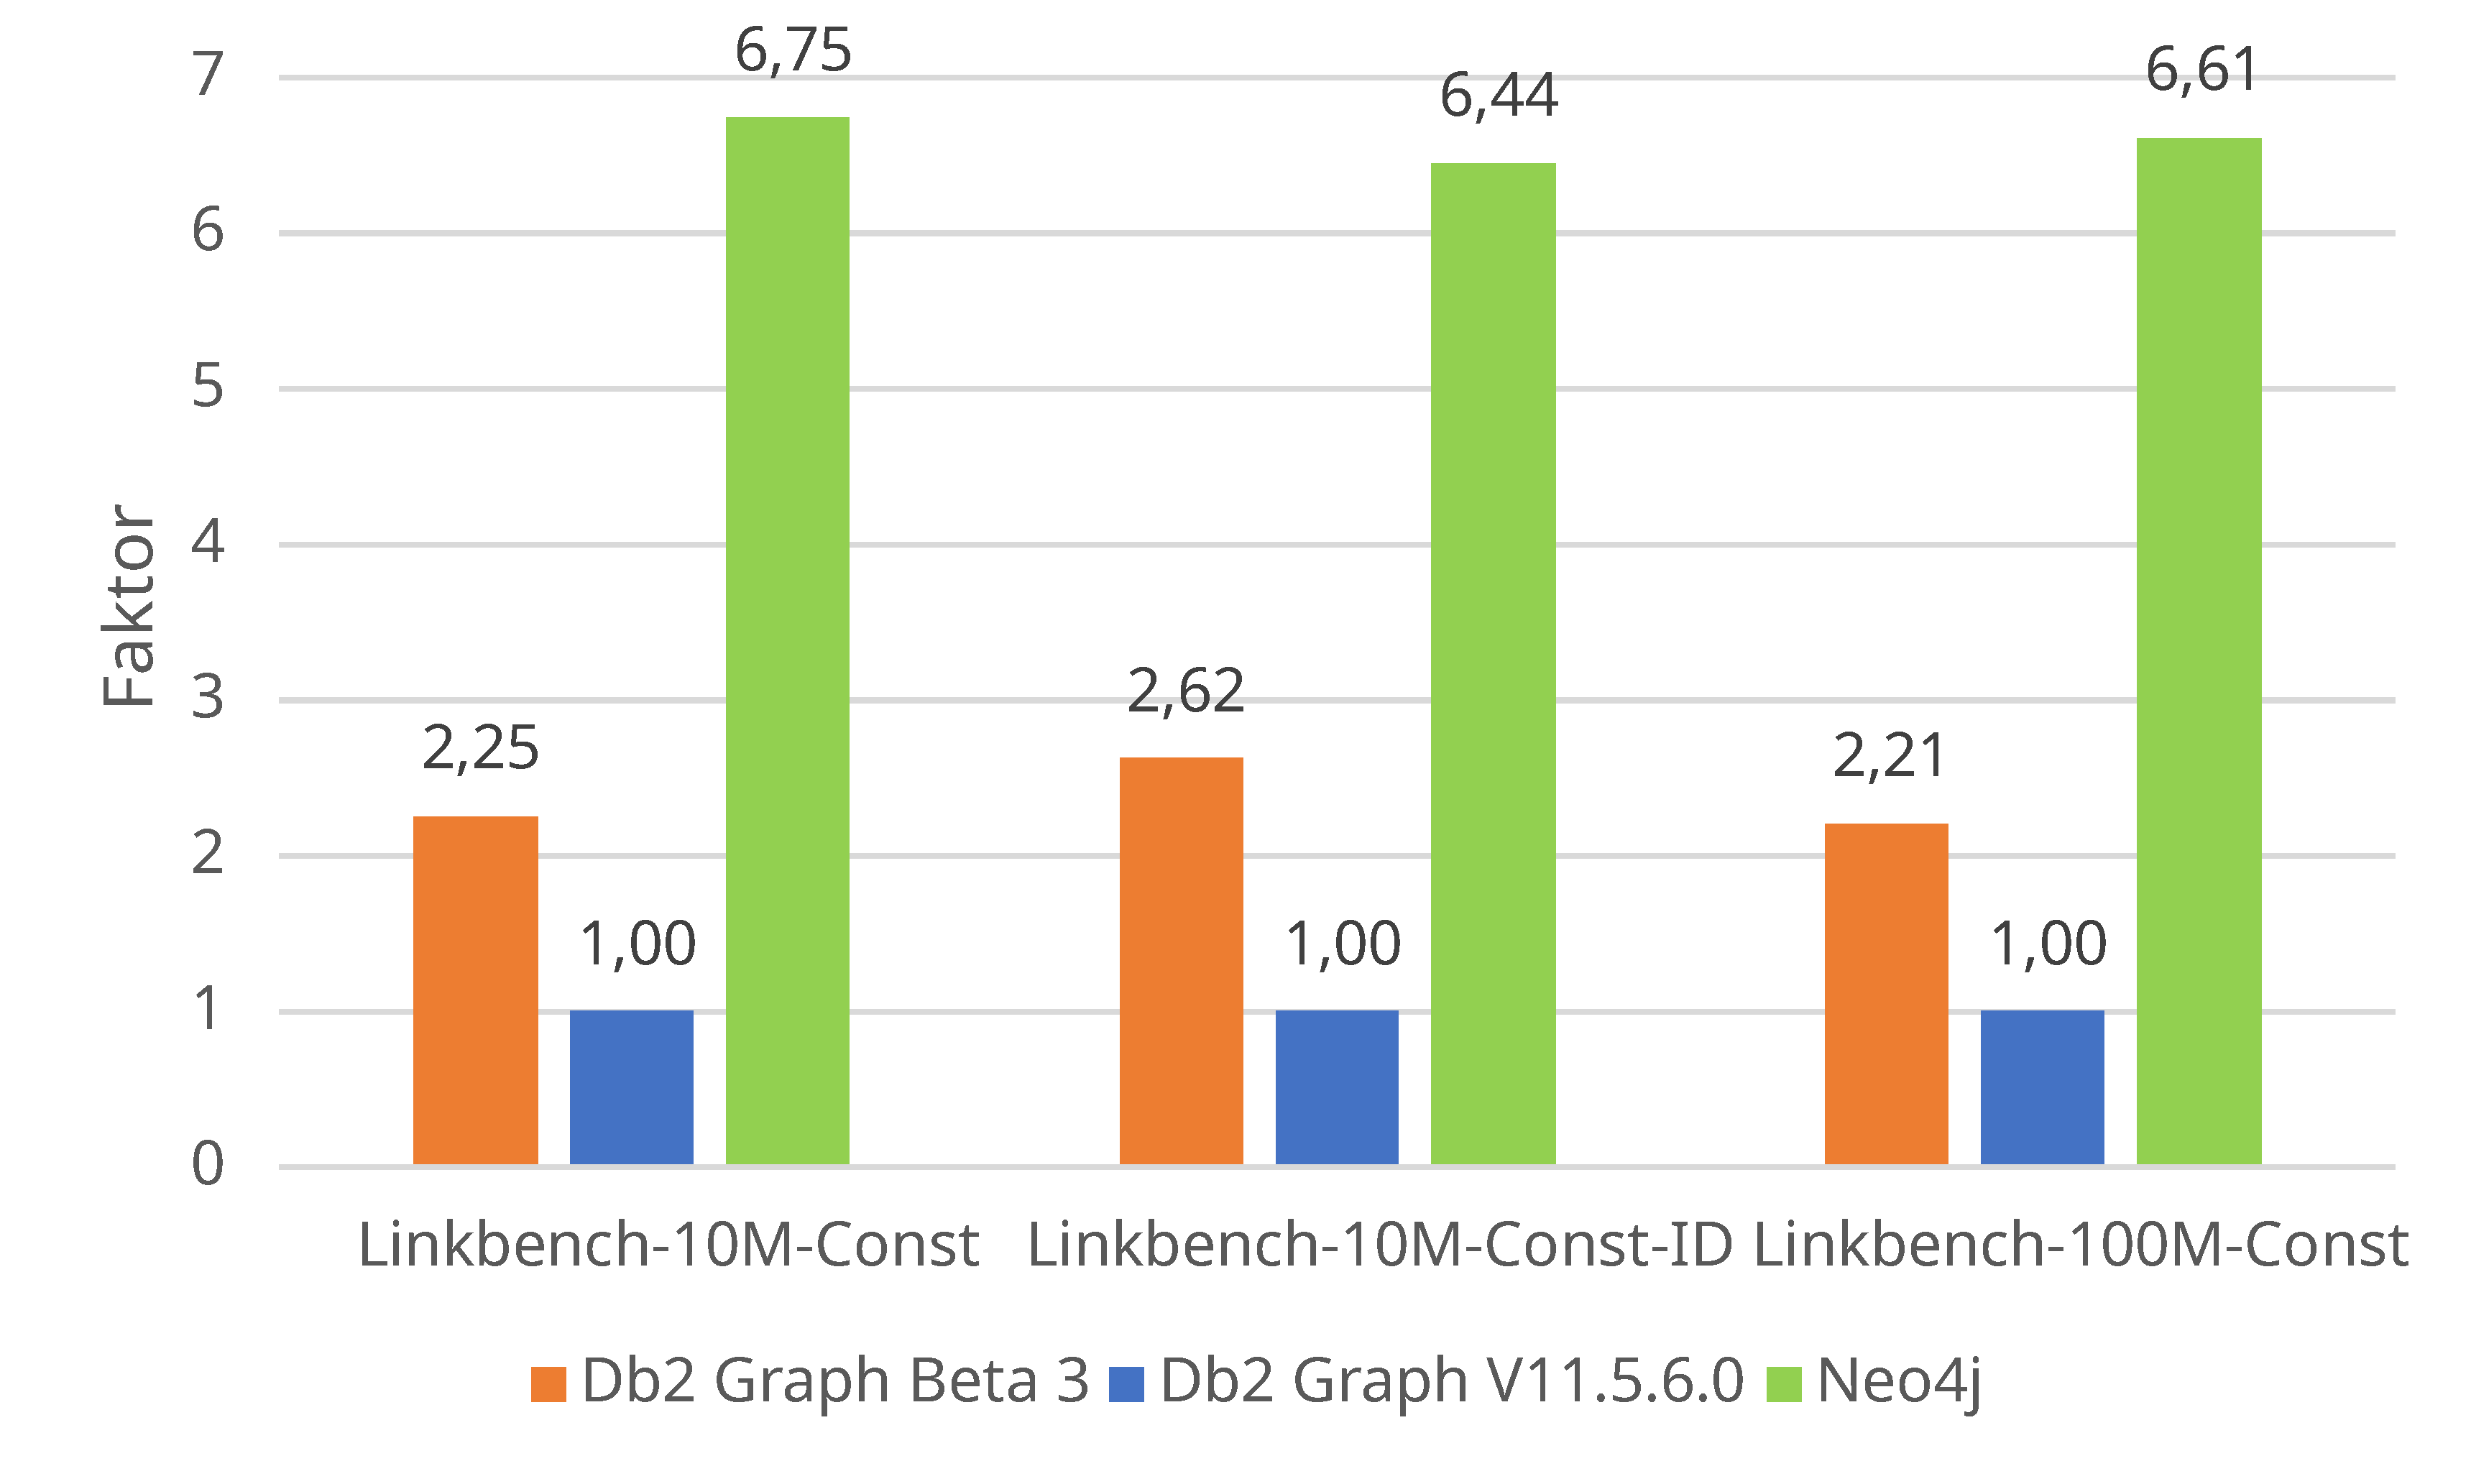
\includegraphics[width=\textwidth]{images/diagramme/faktor_durchschittlicher_durchsatz_const.pdf}
    \caption{Performance-Faktor bei Messreihen mit konstant-verteilten Datensätzen}
    \label{fig:faktor:durchsatz:const}
\end{figure}

\begin{figure}[!ht]
    \centering
    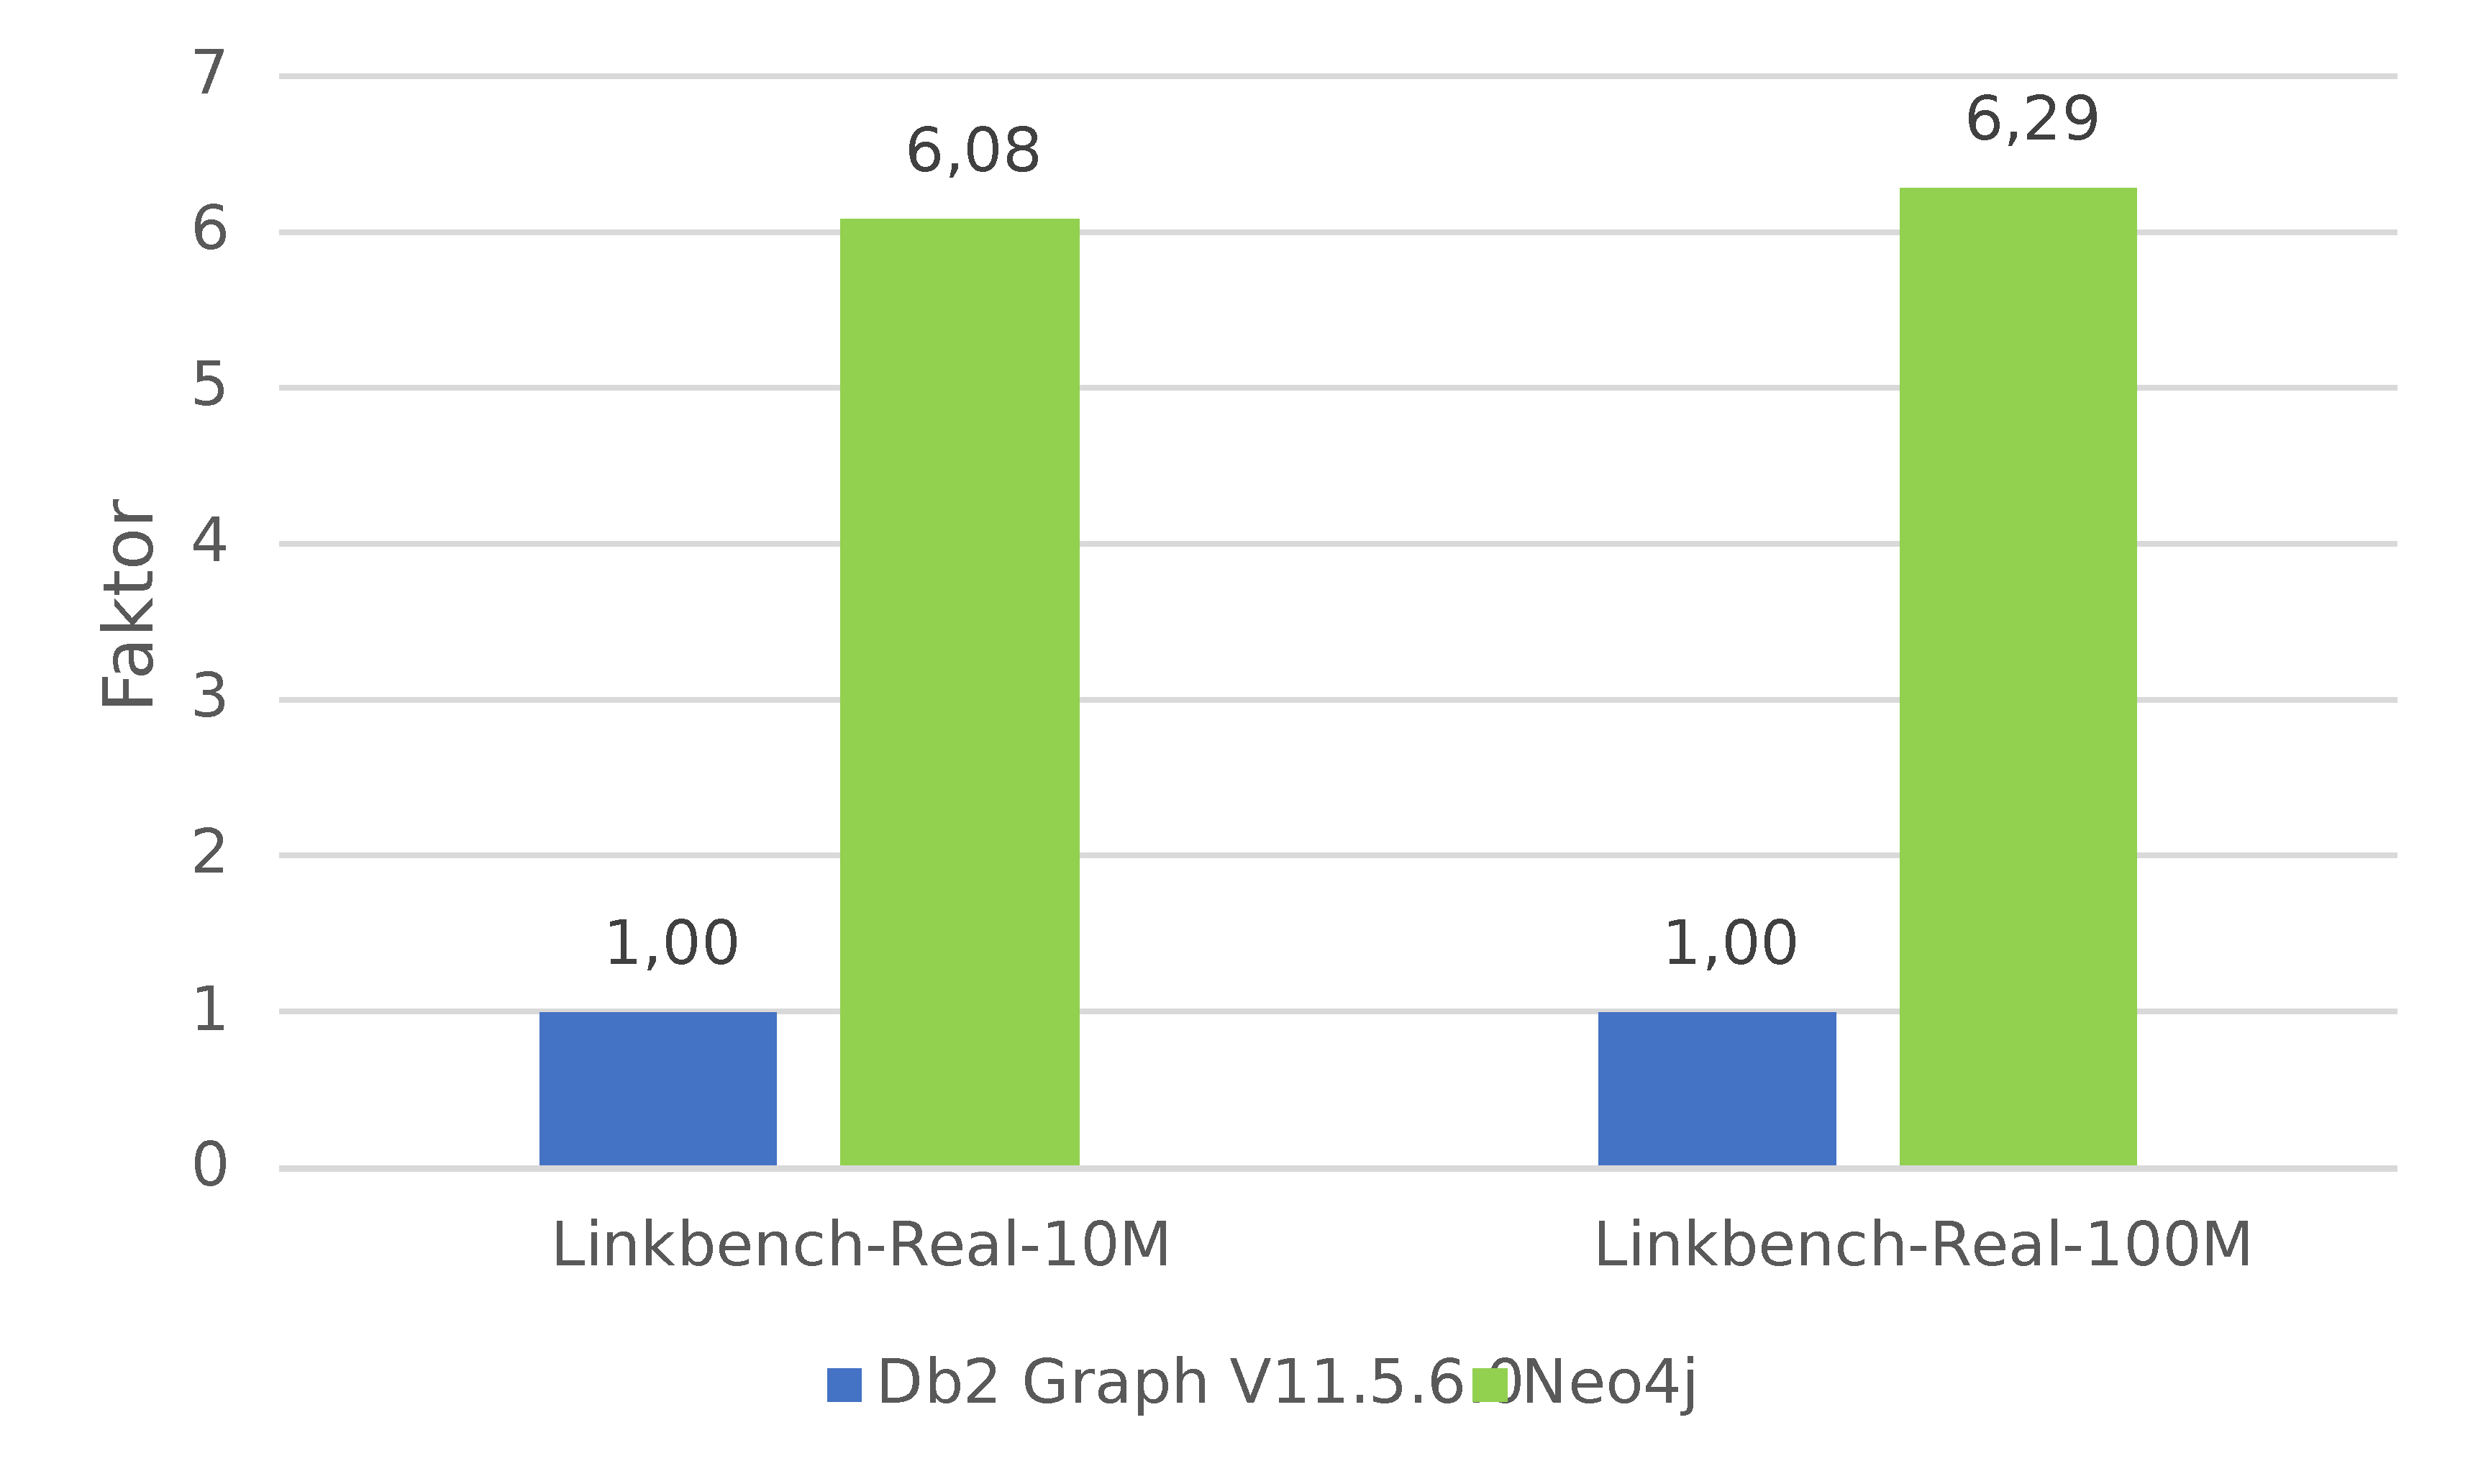
\includegraphics[width=\textwidth]{images/diagramme/faktor_durchschittlicher_durchsatz_real.pdf}
    \caption{Performance-Faktor bei Messreihen mit real-verteilten Datensätzen}
    \label{fig:faktor:durchsatz:real}
\end{figure}

Bei der Analyse der in \autoref{fig:faktor:durchsatz:const} und \autoref{fig:faktor:durchsatz:real} dargestellten Faktoren fällt auf, dass Neo4j immer 6- bis 7-Mal so viele Operationen pro Sekunde bearbeitet wie Db2 Graph bei den jeweiligen Messreihen, was einen gewaltigen Performance-Unterschied zwischen Db2 Graph V11.5.6.0 offenbart. Der Performance-Unterschied zwischen Db2 Graph Beta 3 und Neo4j um ein zwei- bis dreifaches bei den Faktoren in \autoref{fig:faktor:durchsatz:const} ist hier etwas geringer.

So war anfänglich nicht davon auszugehen das Db2 Graph als Grapherweiterung in Kombination mit Db2 Neo4j als natives Graphdatenbanksystem übertrifft. Schließlich verursacht die Kommunikation zwischen Db2 Graph und Db2, die für die Beantwortung einer Anfrage nötig ist, einen Aufwand den Neo4j nicht betreiben muss. Einen Performance-Unterschied um mindestens den Faktor 6 galt es jedoch nicht zu erwarten. 

Eine interessante Gegebenheit, die in der \autoref{fig:faktor:durchsatz:const} beobachtet werden, kann stellt der Fakt dar, dass Db2 Graph Beta 3 als ältere Version von Db2 Graph 2 bis 2,5 Mal mehr Operationen pro Sekunde bewältigen kann, als Db2 Graph V11.5.6.0 (der erste GA Release). Zu Beginn wäre hier eigentlich die Vermutung nahe gelegen, dass V11.5.6.0 als neuere Version, die über mehr Optimierungstechniken verfügt als Beta 3, eine höhere Performance aufweist. Dies ist allerdings nicht der Fall. 

Dabei gilt es hingegen zu beachten, dass Db2 Graph Beta 3 trotz der höheren Performance bei den Messreihen mit konstant-verteilten Datensätzen nicht als allgemein performantere Version von Db2 Graph einzustufen ist. Schließlich spielt sie bei den Messreihen mit real-verteilten Datensätzen keine Rolle, da sie für den Einsatz dort aufgrund fehlender Optimierungstechniken derart ungeeignet ist, dass das Erzielen von Ergebnissen im Rahmen des üblichen Zeitraums nicht möglich ist.

\section{Umgang mit Ergebnismengen}
\label{auswertung:ergebnismenge}
Bei der Untersuchung der Ergebnismenge bei den Messreihen mit real-verteilten Datensätzen wird bereits in \autoref{ergebnisse:10m_real} und \autoref{ergebnisse:100m_real} ein kurzer Überblick über das jeweilige Verhalten bezüglich beim Durchsatzes gegeben. Wie große der verhältnismäßige Einbruch des Durchsatzes und entsprechend auch der Performance, bei einer variierenden oberen Grenze für die Anzahl an Elementen in einer Ergebnismenge ist, lässt sich an den Abbildungen, die absolute Zahlen präsentieren, nicht ablesen. Schließlich bewegen sich die Datenbanksysteme mit beispielsweise 15.742 und 2.466 Operationen pro Sekunde in \autoref{ergebnisse:10m_real} in anderen Größenordnung, werden aber in derselben Grafik abgebildet. 

Um nun der Frage auf den Grund zugehen: \textit{Welches Datenbanksystem bei einem steigenden Range-Limit den verhältnismäßig größeren Performance-Einbruch aufweist?}, wird in \autoref{fig:einbruch:durchsatz:10m} und \autoref{fig:einbruch:durchsatz:100m} dargestellt, wie viele Prozent des Durchsatzes bei einem steigenden Range-Limit noch erreicht werden können. Der Wert für \texttt{getLinkList} mit einem Range-Limit von 100 repräsentiert dabei jeweils 100 \% des Durchsatzes von Neo4j oder Db2 Graph. So sinkt beispielsweise der Durchsatz bei Neo4j in \autoref{fig:einbruch:durchsatz:10m} bei einem Range-Limit von 10.000 auf lediglich 69,74 \% des bei einem Range-Limit von 100 erzielten Durchsatzes. 

Bei der Betrachtung des Kurvenverlaufs in \autoref{fig:einbruch:durchsatz:10m} und \autoref{fig:einbruch:durchsatz:100m} fällt auf das der Durchsatz bei Neo4j eher linear aussieht, während Db2 Graph bei einem Range-Limit von 10.000 jeweils einen Knick aufweist. 

Des Weiteren ist erkennbar, dass der Performance-Einbruch bei Db2 Graph V11.5.6.0 bei einem steigenden Range-Limit immer geringer zu sein scheint, als bei Neo4j. So weist V11.5.6.0 bei einem Range-Limit von 100.000 noch 54,18 \% des Durchsatzes auf den es bei einem Range-Limit von 100 erreicht hat. Neo4j hingegen erlangt bei 100.000 lediglich 43,29 \% des Durchsatzes den es erreicht, wenn die Ergebnismenge auf eine obere Grenze von 100 Elemente begrenzt wird. 

So beträgt der Unterschied zwischen Db2 Graph und Neo4j bei einem Range-Limit von 100.000 ca. 11 \% zueinander in \autoref{fig:einbruch:durchsatz:10m}, während es bei 10.000 sogar ca. 18 \% sind. Bei einem Range-Limit von 1.000 sind es jedoch lediglich ca. 8 \% Unterschied zueinander. Wobei es bei hier anzumerken gilt, dass Db2 Graph mit 97,58 \% ein außergewöhnlich hohes Ergebnis erreicht. Die in \autoref{fig:einbruch:durchsatz:100m} dargestellten Werte bestätigen dabei grob die Beobachtungen aus \autoref{fig:einbruch:durchsatz:10m}. So weichen die Werte in den beiden Abbildungen (\autoref{fig:einbruch:durchsatz:10m} und \autoref{fig:einbruch:durchsatz:100m}) höchstens um bis zu 2 \% voneinander ab. 

\begin{figure}[!ht]
    \centering
    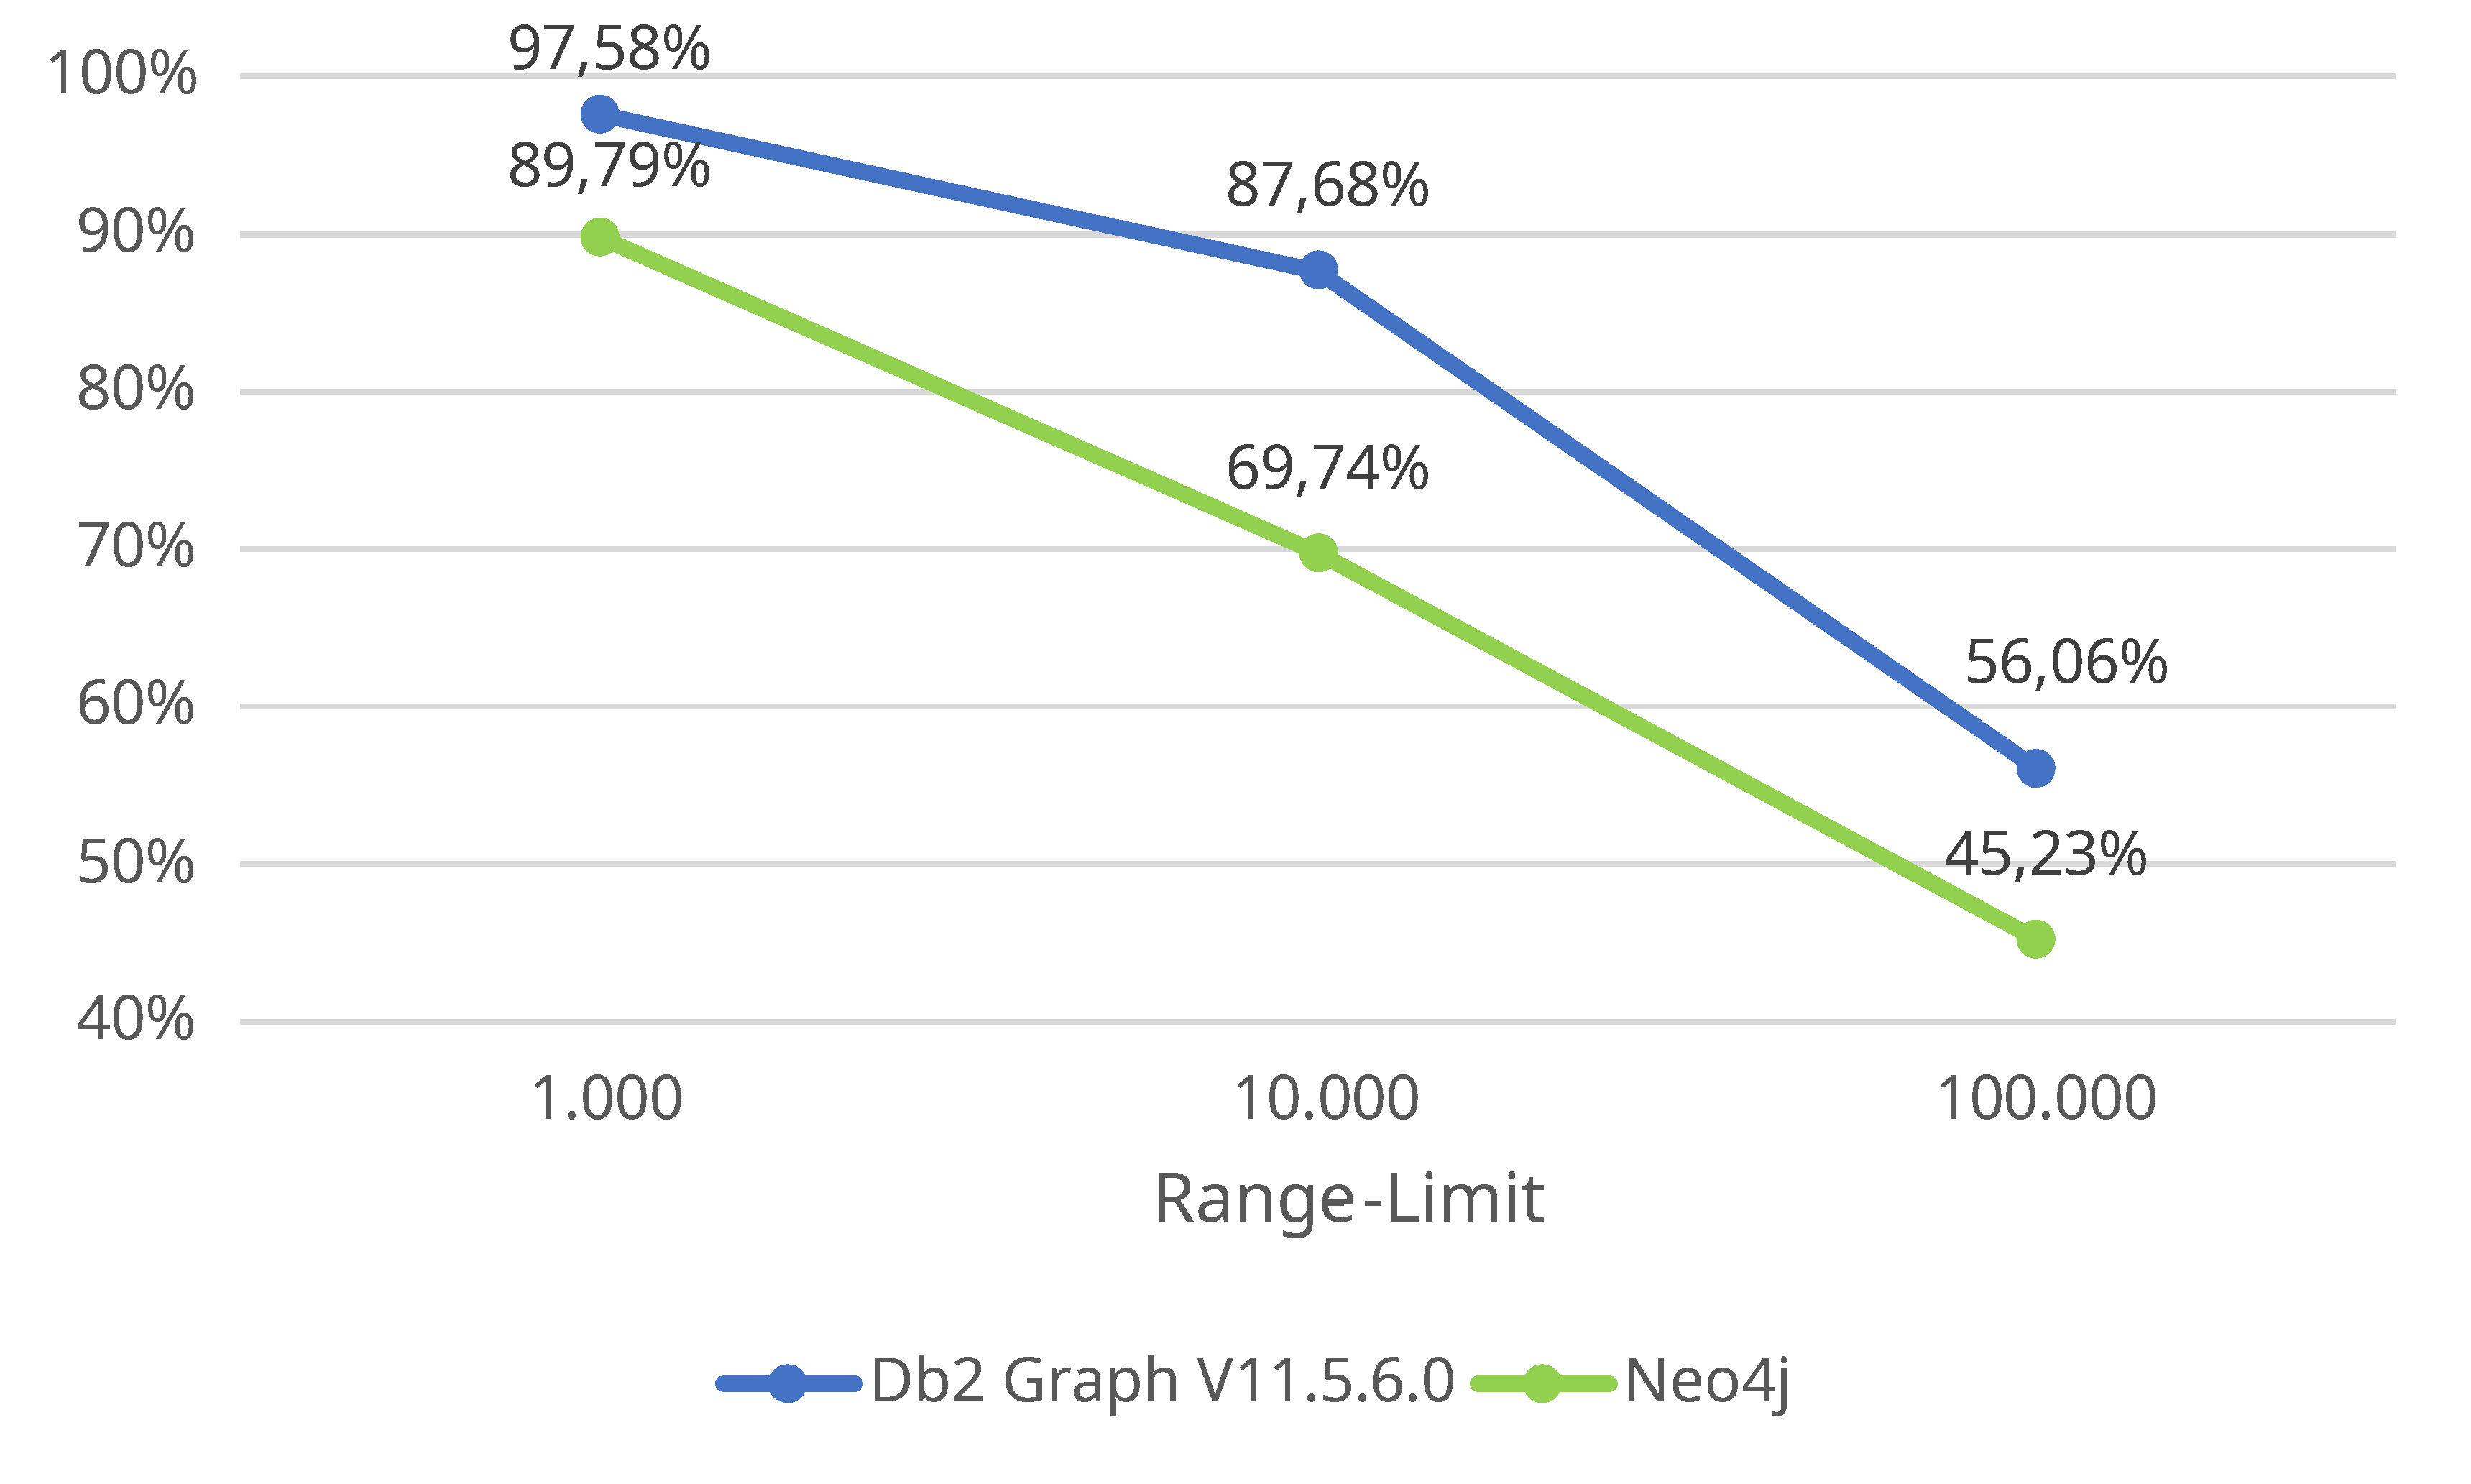
\includegraphics[width=\textwidth]{images/diagramme/limit_relative_durchsatz_real_10m.pdf}
    \caption{Linkbench-10M-Real Durchsatz gemessen an getLinkList(100)}
    \label{fig:einbruch:durchsatz:10m}
\end{figure}

\begin{figure}[!ht]
    \centering
    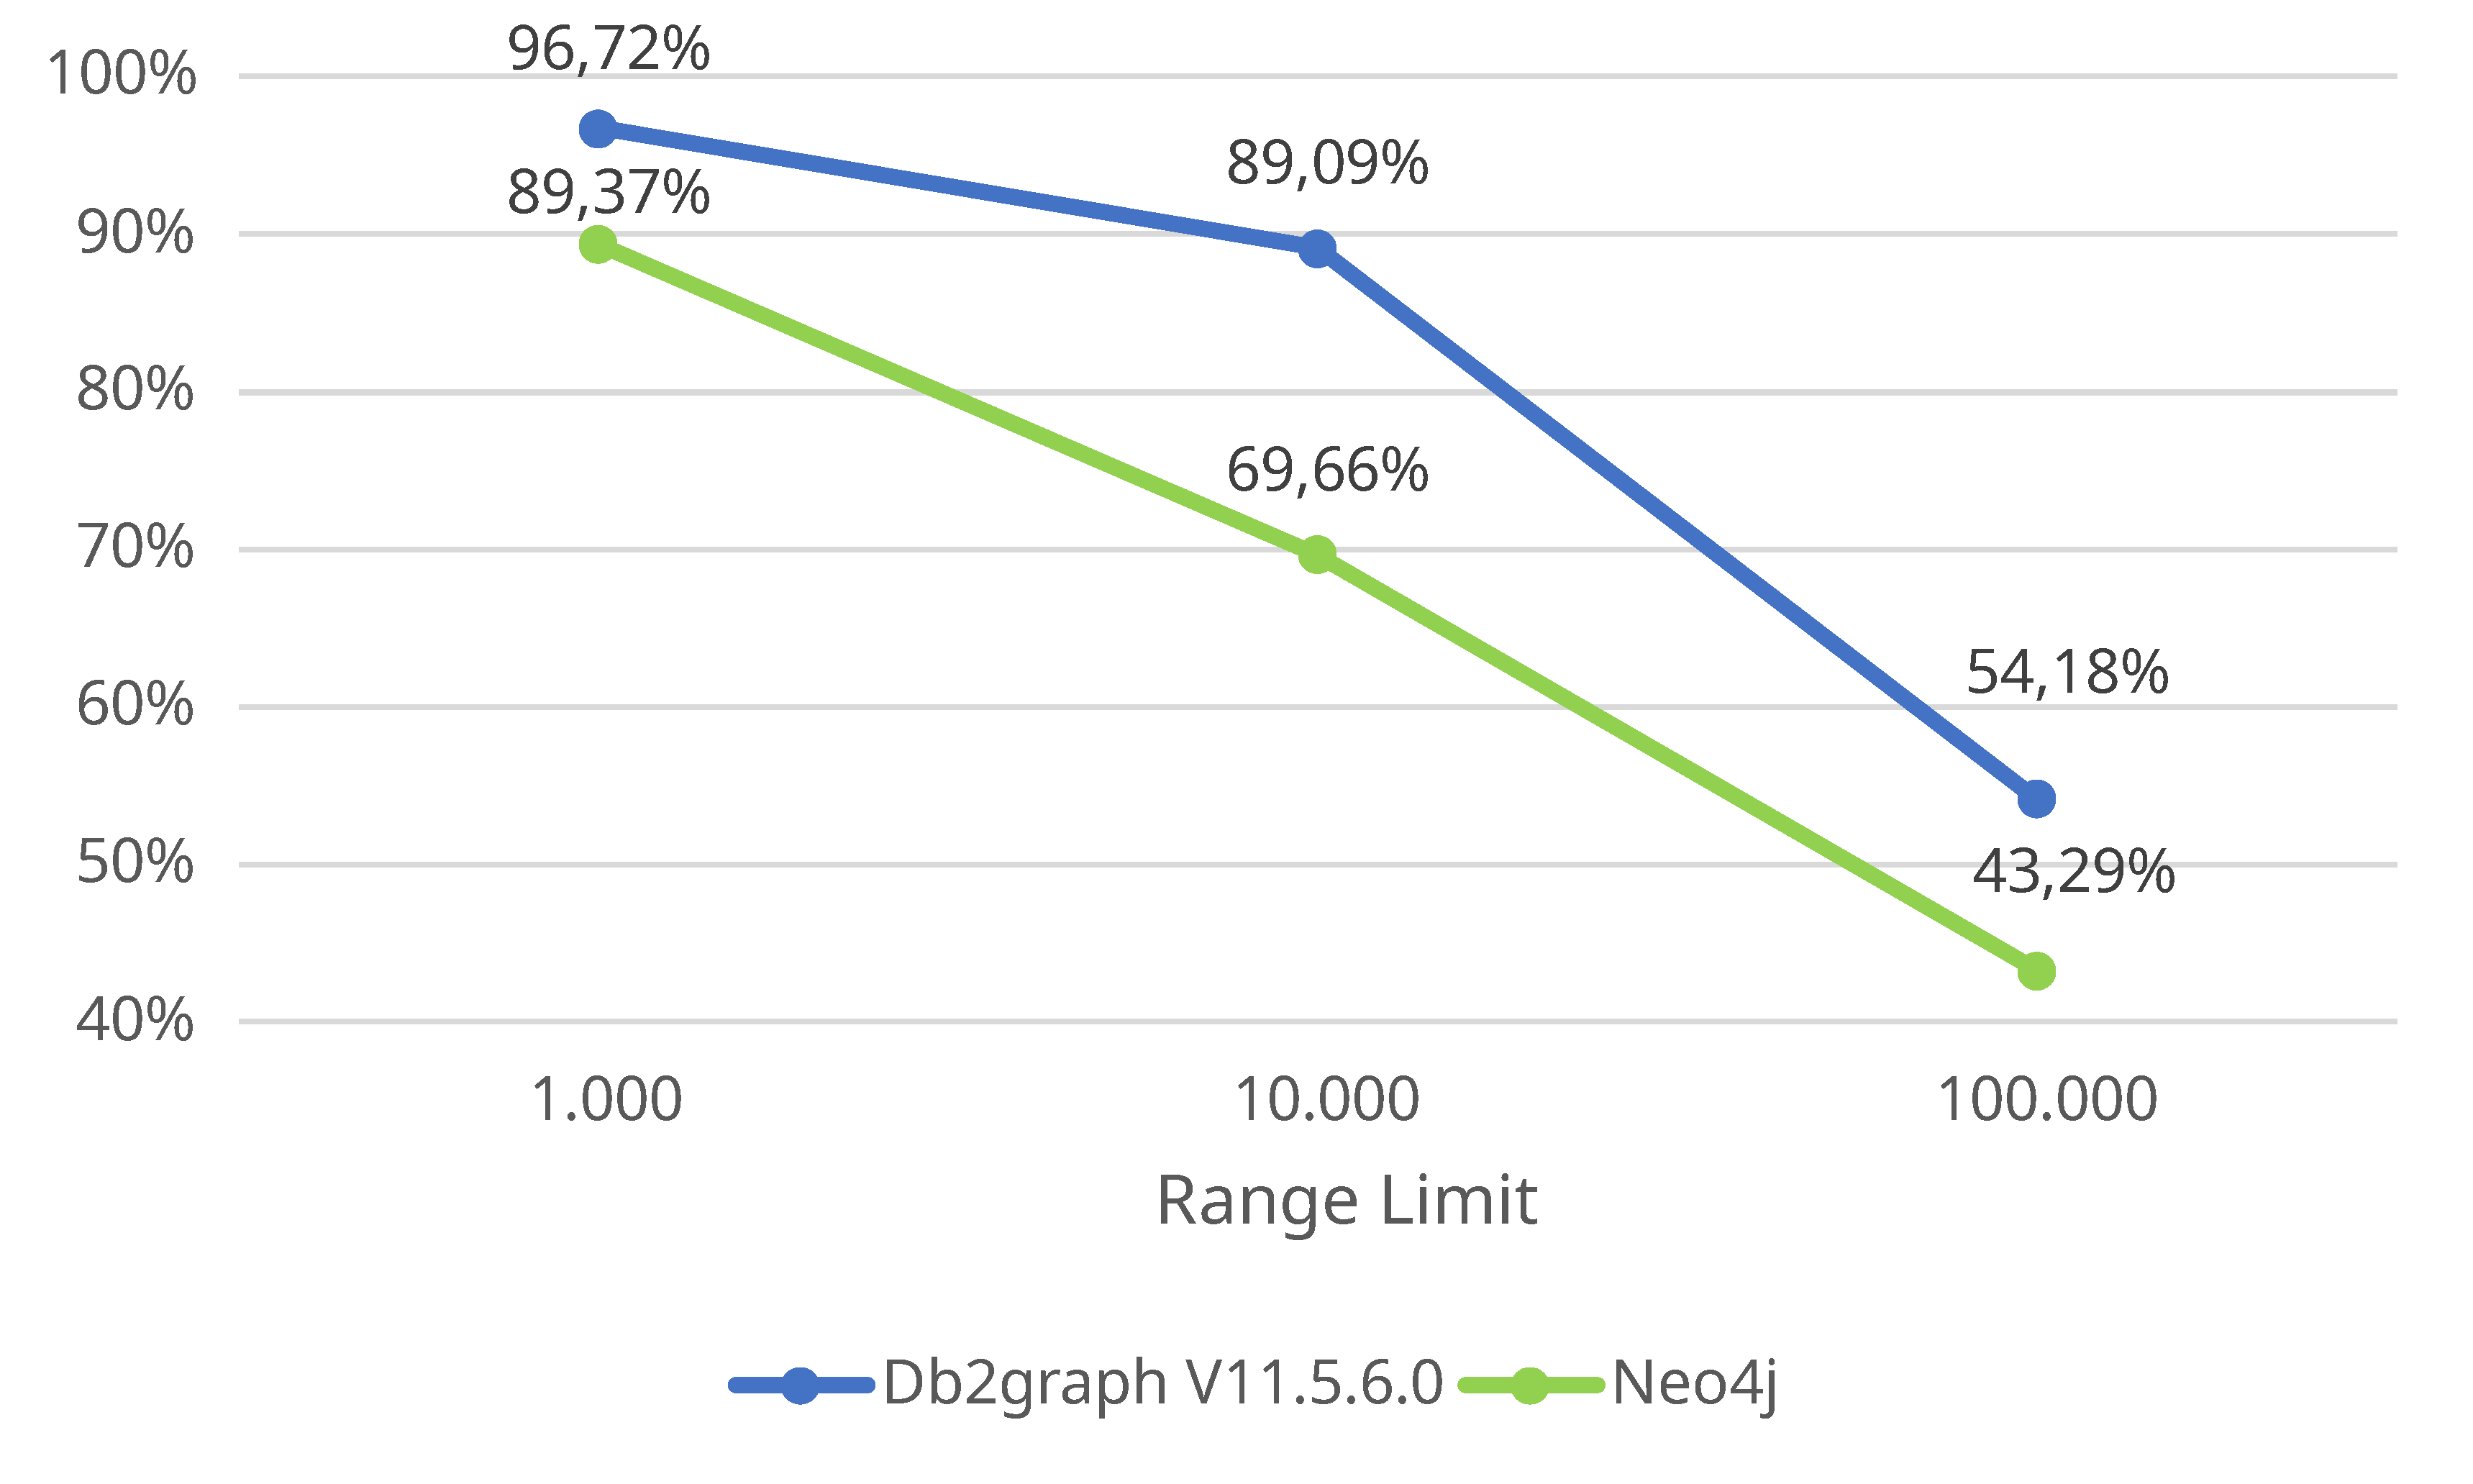
\includegraphics[width=\textwidth]{images/diagramme/limit_relative_durchsatz_real_100m.pdf}
    \caption{Linkbench-100M-Real Performance gemessen an getLinkList(100)}
    \label{fig:einbruch:durchsatz:100m}
\end{figure}

Schlussendlich kann basierend auf \autoref{fig:einbruch:durchsatz:10m} und \autoref{fig:einbruch:durchsatz:100m} das Fazit gezogen werden, dass der Performance Einbruch beim Umgang mit größeren Ergebnismengen bei Neo4j nicht nur in absoluten Zahlen ausfällt, sondern auch im Verhältnis.

\section{Einfluss der Datensatzgröße}
\label{auswertung:groesse}
Im Rahmen dieses Abschnitts wird genauer untersucht, welchen Einfluss die Größe eines Datensatzes auf konstant- oder real-verteilten Datensätze hat. Um dies bei den Datenbanksystemen zu identifizieren, wird der relative Unterschied zwischen den Durchsatzergebnisse zwischen den Linkbench-10M und Linkbench-100M Datensätzen ermittelt. Die jeweiligen Durchsatzergebnisse die mit Linkbench-10M Datensätzen erzielt werden, werden dabei als 100 \% betrachtet. An diesen 100 \% wird im nächsten Schritt der Durchsatz bei den Linkbench-100M Datensätzen gemessen. Die prozentuale Abweichungen zwischen den Datensätzen werden dabei in \autoref{fig:durchsatz:10m_vs_100m:const} und \autoref{fig:durchsatz:10m_vs_100m:real} dargestellt.

\begin{figure}[!ht]
    \centering
    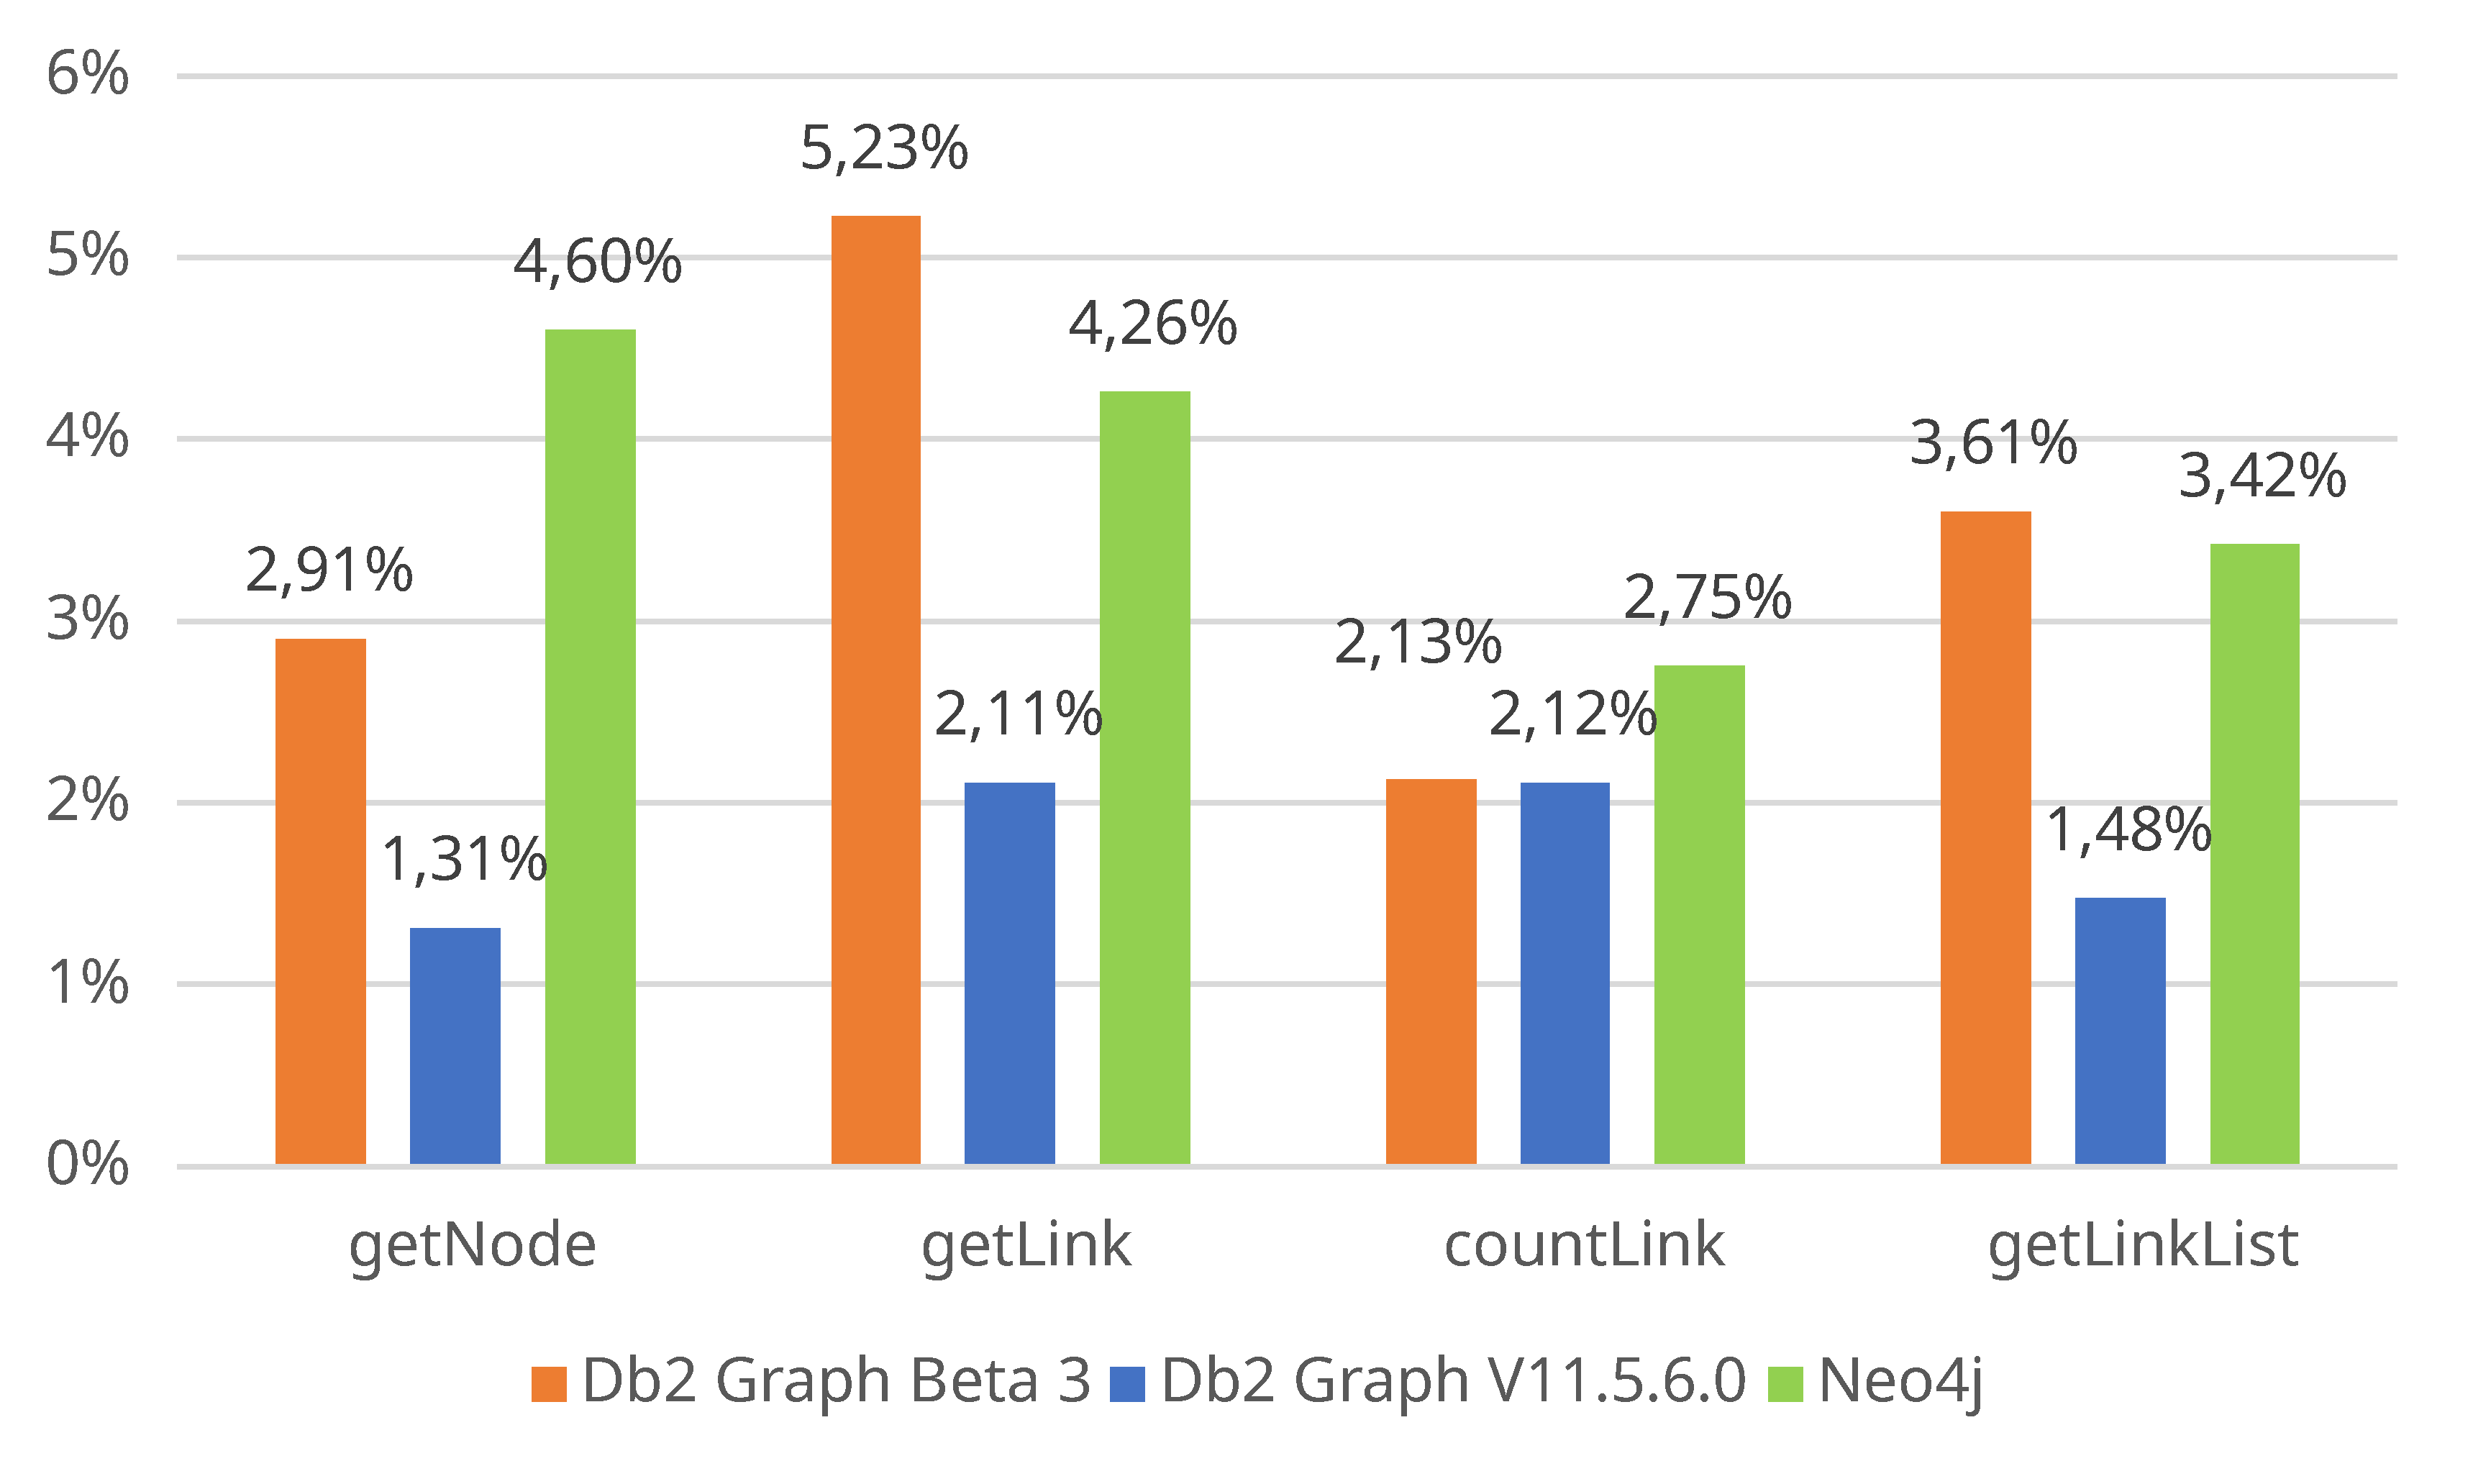
\includegraphics[width=\textwidth]{images/diagramme/difference_durchsatz_const_10m_vs_100m.pdf}
    \caption{Unterschied Durchsatz Linkbench-10M vs. Linkbench-100M (Const)}
    \label{fig:durchsatz:10m_vs_100m:const}
\end{figure}

\begin{figure}[!ht]
    \centering
    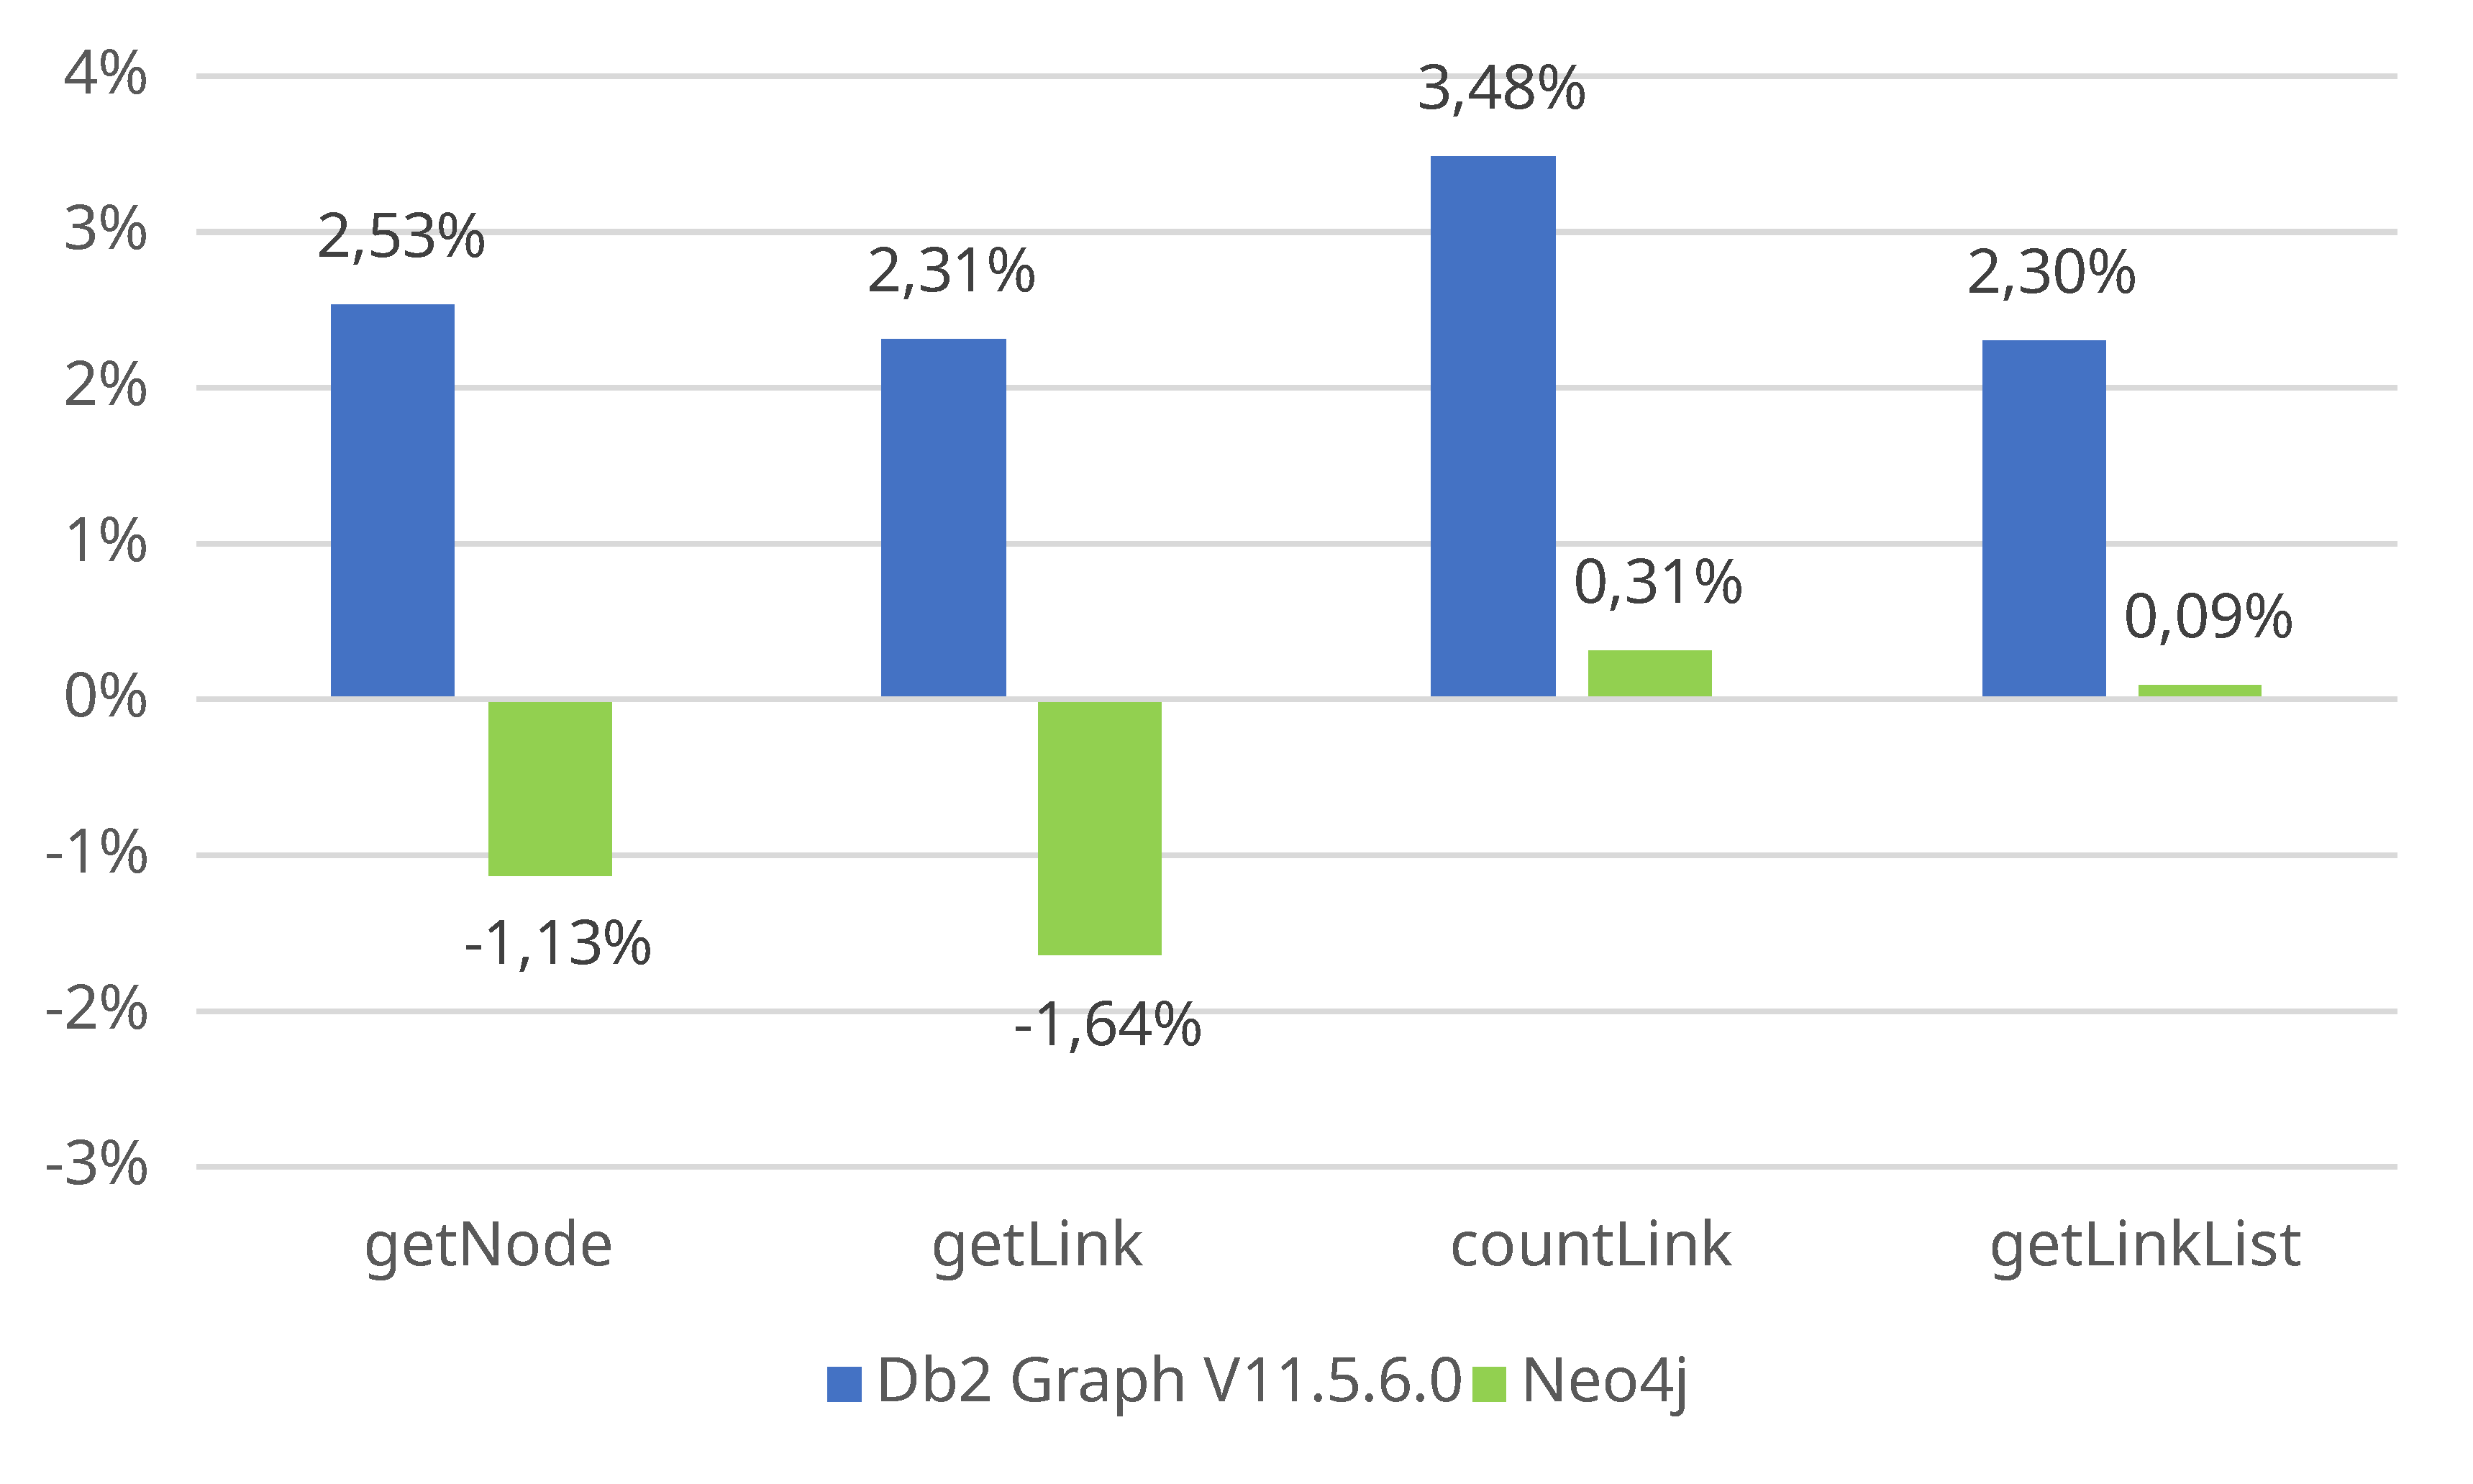
\includegraphics[width=\textwidth]{images/diagramme/difference_durchsatz_real_10m_vs_100m.pdf}
    \caption{Unterschied Durchsatz Linkbench-10M vs. Linkbench-100M (Real)}
    \label{fig:durchsatz:10m_vs_100m:real}
    \vspace{1em}
    \textit{Bei den hier abgebildeten Werten für getLinkList, handelt es sich um Werte, die mit einem Range-Limit von 100 erzielt werden.}
\end{figure}

So gilt es den in \autoref{fig:durchsatz:10m_vs_100m:const} bei \texttt{getNode} für Db2 Graph Beta 3 angegebenen Wert von 2,91 \% so zu verstehen, dass der Durchsatz bei Linkbench-100M um diesen Prozentsatz geringer ausfällt als bei derselben Messung mit dem Linkbench-10M. Db2 Graph Beta 3 erreicht also bei der Messreihe \nameref{ergebnisse:100m_const} lediglich 97,09 \% des Durchsatzes von der Messreihe \nameref{ergebnisse:10m_const}, wodurch sich der Unterschied von 2,91 \% bei \texttt{getNode} ergibt.

Die in \autoref{fig:durchsatz:10m_vs_100m:const} für konstant-verteilte Datensätze dargestellten Ergebnisse zeigen hier einen konstantes Bild über alle Datenbanksysteme hinweg. So weisen alle Messergebnisse, egal welches Datenbanksystem oder welche Operation, eine positive prozentuale Abnahme auf. Dies bedeutet, dass sich wie bei größeren Datensätzen erwartet, alle Durchsatzergebnisse bei \nameref{ergebnisse:100m_const} im Verhältnis zu \nameref{ergebnisse:10m_const} niedriger ausgefallen sind. Neo4j weist dabei mit 1,31 \% bis 2,12 \% den geringsten Performance-Einbruch auf. Neo4j und Db2 Graph V11.5.6.0 hingegen weisen deutlich höhere Performance-Einbrüche bei dem größeren Datensatz auf mit jeweils 4,60 \% (\texttt{getNode}) und 5,23 \% (\texttt{getLink}). 

Die in \autoref{fig:durchsatz:10m_vs_100m:real} abgebildeten Ergebnisse überraschen hingegen. Die Ergebnisse für Neo4j bewegen sich hier bei \texttt{getNode} und \texttt{getLink} im negativen Bereich. Dies bedeutet, dass für Neo4j bei diesen Operationen in \nameref{ergebnisse:100m_real} ein höherer Durchsatz erzielt werden konnte, als beim kleineren Datensatz in \nameref{ergebnisse:10m_real}, was der bereits zuvor geäußerten These, dass größere Datensätze einen geringeren Durchsatz beziehungsweise eine geringere Performance aufweisen widerspricht. Auch gibt es bei den Messungen keinerlei Anhaltspunkte, warum dieses Phänomen bei Neo4j auftritt. Alle anderen Wert von Neo4j und Db2 Graph V11.5.6.0 weisen hingegen positive Performance-Einbrüche auf.

Bezüglich der Höhe der Abweichungen kann aus \autoref{fig:durchsatz:10m_vs_100m:real} abgeleitet werden, dass Db2 Graph mit Abweichungen zwischen 2,3 \% und 3,48 \% eine höhere Abweichung aufweist als Neo4j, das sich im Bereich von 0,09 \% bis (-)1,64 \% bewegt. 

\section{Ressourcenauslastung}
\label{auswertung:ressourcenauslastung}

Im Rahmen dieses Kapitels werden einige NMON-Statistiken zur Ressourcenauslastung ausgewertet. Dabei wird die CPU- und IO-Aus\-last\-ung genauer untersucht und die darin erkennbaren Trends und Unterschiede zwischen den Datenbanksystemen angesprochen. 

Ziel dieses Abschnitts ist es dabei die Ressourcenauslastung der Datenbanksysteme miteinander zu Vergleichen und möglicherweise einen Hinweis darauf zu finden, warum der Performance-Unterschied zwischen Db2 Graph Beta 3 und V11.5.6.0 mit einem Unterschied des Faktors 2,25 derart signifikant ausfällt. 

Für den Vergleich der Datenbanksysteme wird dabei exemplarisch deren Ressourcenauslastung bei der Operation \texttt{getNode} in den Messreihen \autoref{ergebnisse:10m_const} und \autoref{ergebnisse:10m_real} herangezogen. Denn die Abbildung und Auswertung aller 64 Statistiken, die bei der Performance-Analyse durch das Werkzeug NMON aufgezeichnet werden, wäre hier aufgrund des Umfangs nicht zielführend. Alle Statistiken die im Rahmen der Arbeit aufgezeichnet werden, werden allerdings als NMON-Dateien dem digitalen Anhang der Arbeit beigelegt, sodass alle erzielten Statistiken einsehbar sind.

Bei der Auswertung der Statistiken gilt es dabei allerdings zu beachten, dass die CPU-Auslastung und Anzahl an IO-Ope\-ra\-ti\-on\-en (Disk xfers) pro Sekunde, die von den Abbildungen dieses Abschnitts aufgeführt werden, immer die Auslastung der ganzen Maschine, in der die Messungen stattfinden, wiedergeben. So gilt es dabei auch immer im Auge zu behalten, dass beispielsweise das Betriebssystem selbst und andere kleinere Server-Prozesse ebenfalls geringfügig etwas zur CPU- und IO-Aus\-last\-ung beitragen.  

\subsection{Linkbench-10M-Const}
\label{auswertung:ressourcenauslastung:const}
Bei der Auswertung der Ressourcenstatistiken bei dieser Messreihe kann mit Hinblick auf die Statistiken identifiziert werden, dass die CPU-Auslastung bei Neo4j (\autoref{fig:nmon:10m:const:neo4j}) am höchsten ist, gefolgt von Db2 Graph Beta 3 (\autoref{fig:nmon:10m:const:beta3}) und mit größerem Abstand Db2 Graph V11.5.6.0 (\autoref{fig:nmon:10m:const:ga}). 

Dabei fällt auf, dass der Unterschied bei der CPU-Auslastung zwischen Neo4j und Db2 Graph Beta 3 mit ca. 5 - 7 \% eher geringer ausfällt, während der Unterschied zwischen Beta 3 und V11.5.6.0 ca. 30 \% umfasst. Dies scheint allerdings ungefähr zu den Beobachtungen in \nameref{auswertung:einordnung} zu passen, wo Beta 3 die 2,25 Performance von V11.5.6.0 aufweist. Schließlich weist Beta 3 in (\autoref{fig:nmon:10m:const:beta3}) mit ca. 69 \% gegenüber der rund 39 \% grob auch beinahe eine doppelte Ressourcenauslastung auf.

Allgemein kann angemerkt werden, dass alle Statistiken eine konstante CPU-Auslastung über den jeweiligen Messzeitraum aufweisen. So zeigt beispielsweise die Aufzeichnung für Neo4j (\autoref{fig:nmon:10m:const:neo4j}) eine andauernde CPU-Auslastung von ca. 76 \% über den Messzeitraum an, bis auf den Beginn und das Ende der Aufzeichnung. Db2 Graph Beta 3 und V11.5.6.0 weisen in ihren jeweiligen Statistiken ein ähnlich konstantes Niveau der CPU-Auslastung auf. 

Wird statt der CPU-Auslastung die Anzahl an IO-Ope\-ra\-ti\-on\-en pro Sekunde in den Ressourcenstatistiken der Datenbanksysteme untersucht, so fällt hierbei auf, dass sich die Skalen und Werte der IO-Aus\-last\-ung (Disk xfers) in \autoref{fig:nmon:10m:const:beta3},\autoref{fig:nmon:10m:const:ga} und \autoref{fig:nmon:10m:const:neo4j} erheblich unterscheiden. Während bei Db2 Graph V11.5.6.0 ca. 7.500 Read- oder Write-Ope\-ra\-ti\-on\-en pro Sekunde auf den Festplattenspeicher durchgeführt werden, sind es bei Neo4j lediglich 2,5 bis 5. 
\begin{figure}[!ht]
    \centering
    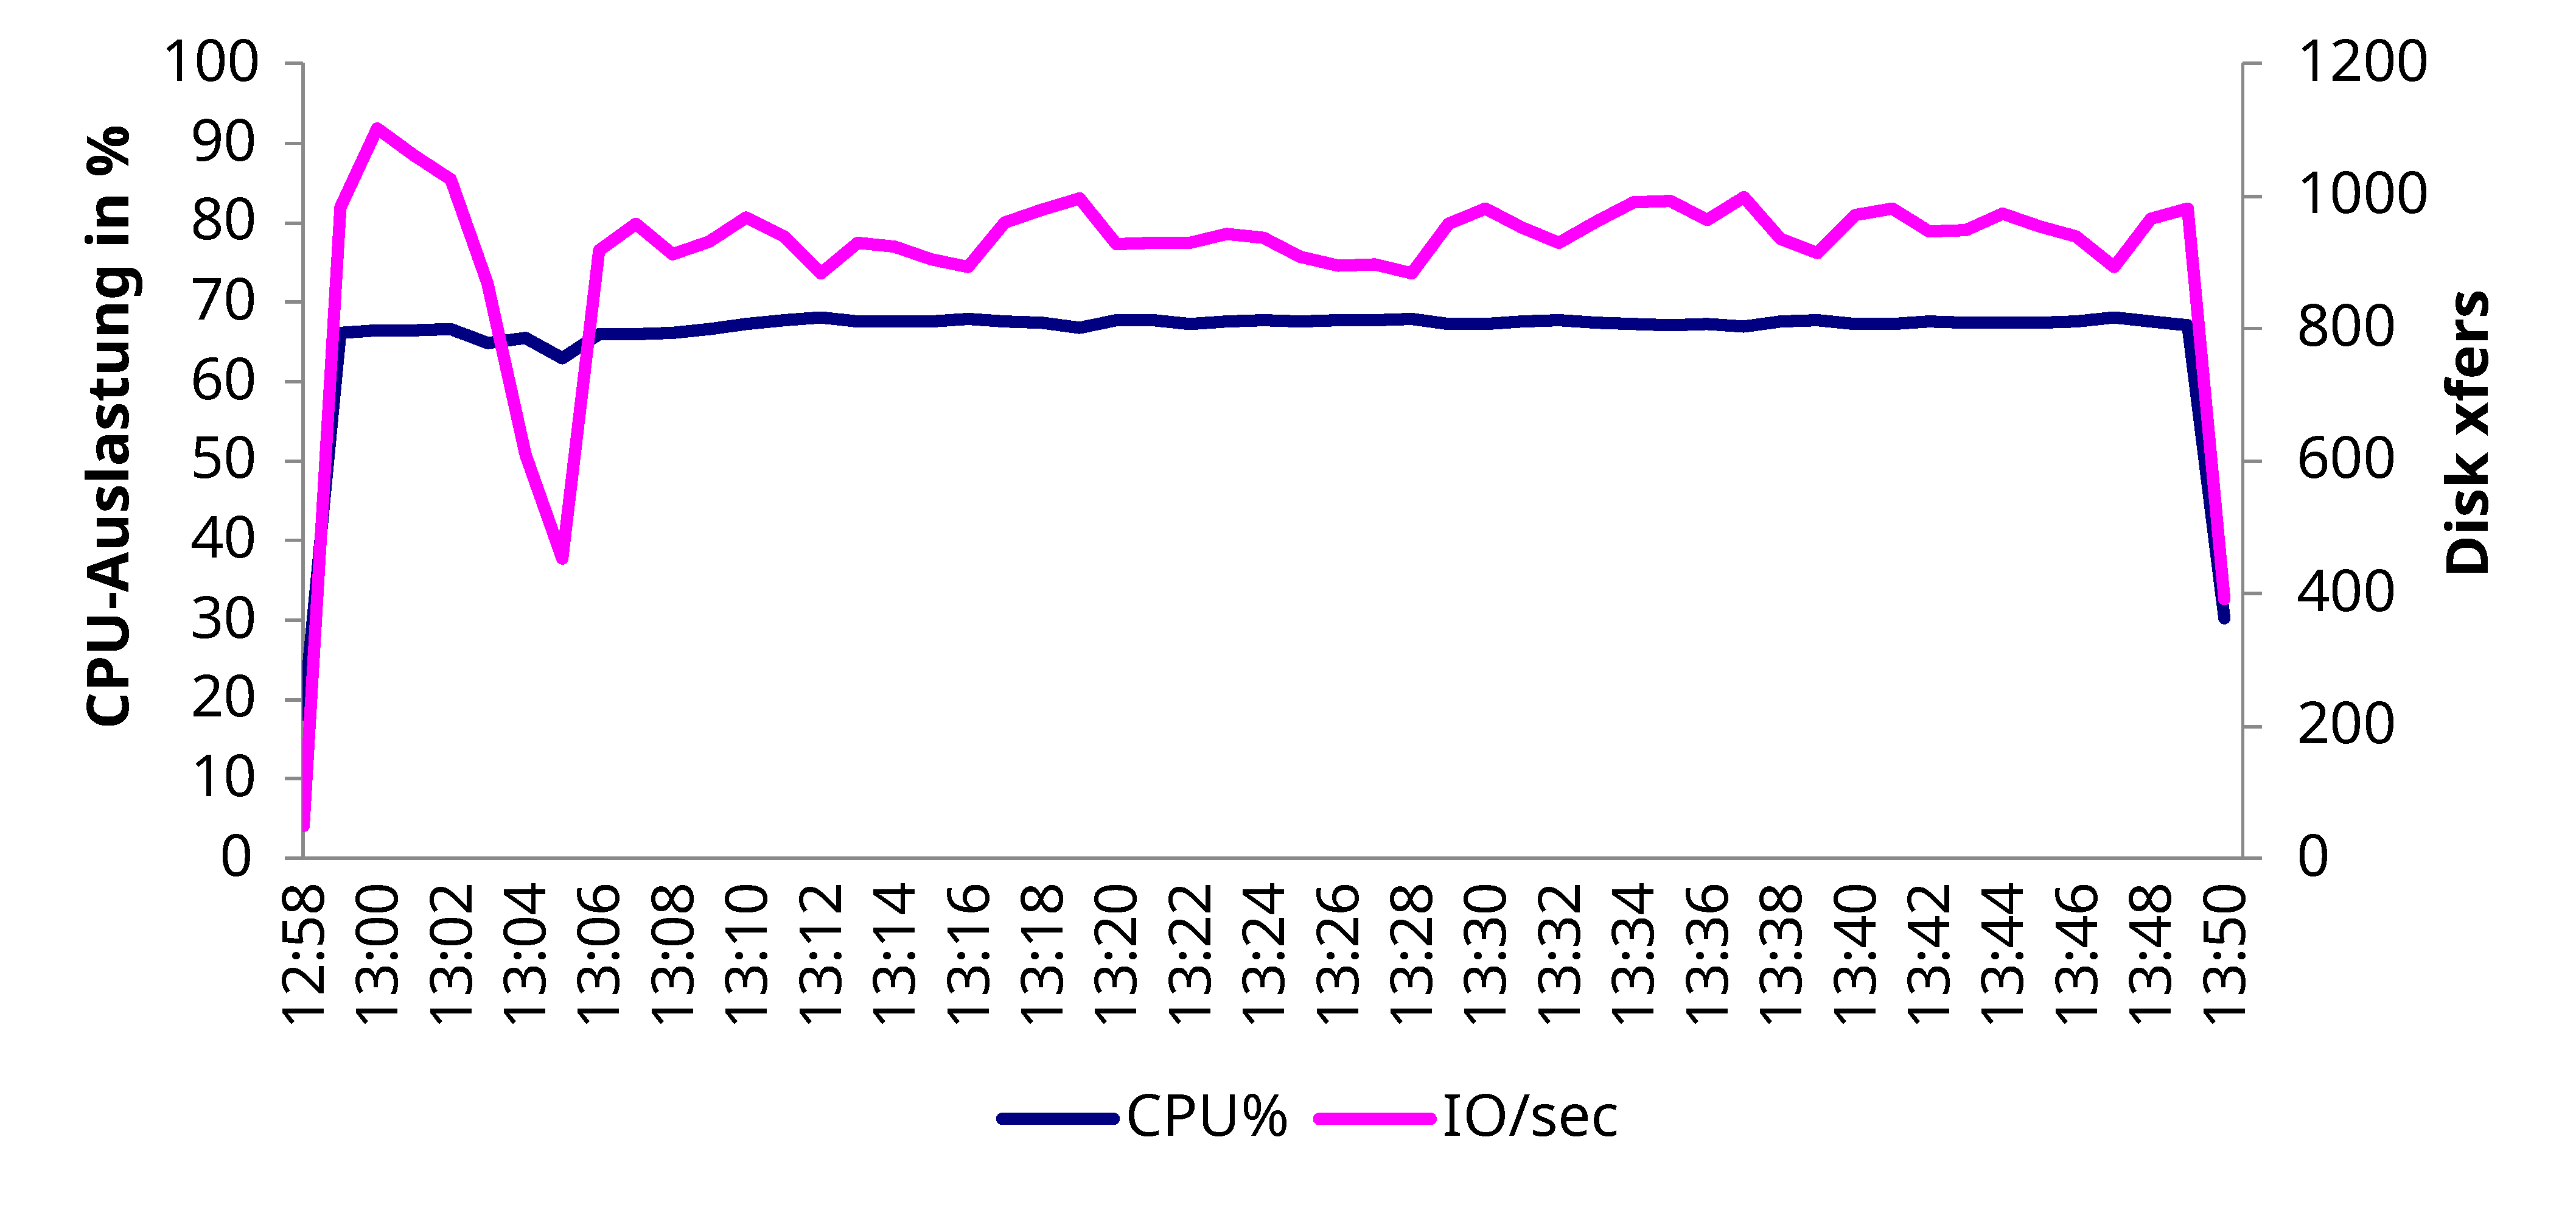
\includegraphics[width=\textwidth]{images/stats/linkbench-10m-const_beta3.pdf}
    \caption{Linkbench-10M-Const Auslastung Db2 Graph Beta 3 (getNode)}
    \label{fig:nmon:10m:const:beta3}
\end{figure}

\begin{figure}[!ht]
    \centering
    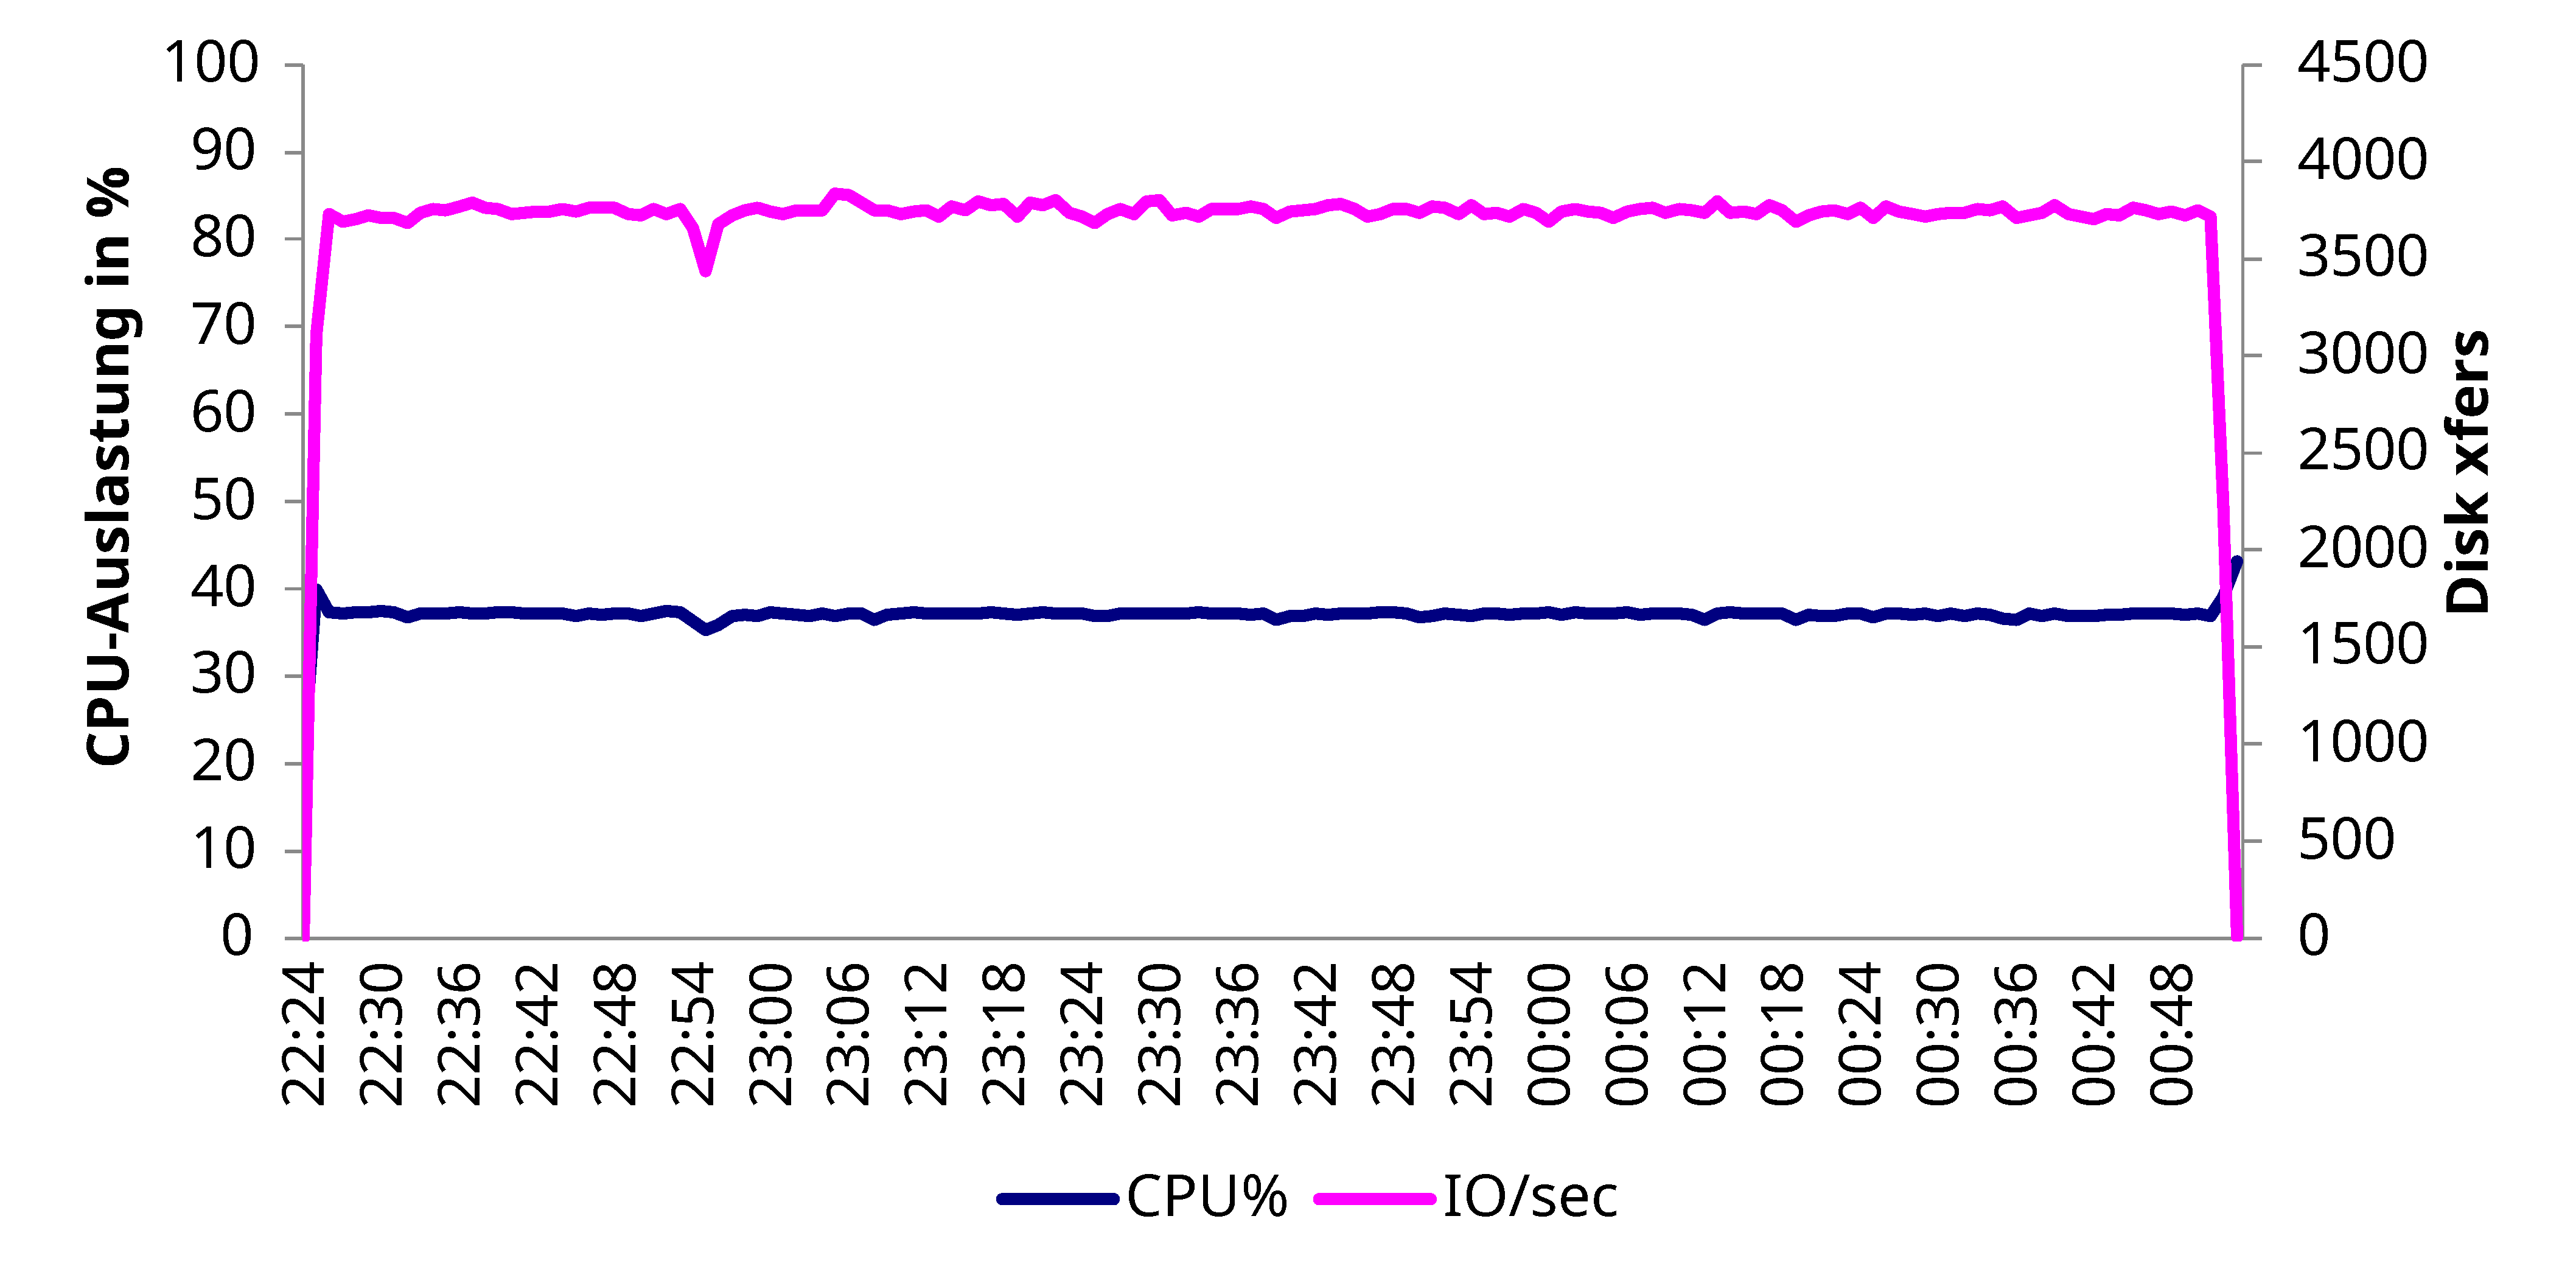
\includegraphics[width=\textwidth]{images/stats/linkbench-10m-const_ga.pdf}
    \caption{Linkbench-10M-Const Auslastung Db2 Graph V11.5.6.0 (getNode)}
    \label{fig:nmon:10m:const:ga}
\end{figure}

Db2 Graph Beta 3 bewegt sich hingegen mit durchschnittlich ca. 900 IO-Ope\-ra\-ti\-on\-en pro Sekunde im Mittelfeld. Damit liegt Beta 3 zwar unterhalb von V11.5.6.0, weist allerdings immer noch mehr als das 100-fache der IO-Ope\-ra\-ti\-on\-en pro Sekunde auf wie Neo4j im Schnitt. Die signifikant geringere IO-Aus\-last\-ung könnte sich dabei damit erklären lassen, dass Neo4j scheinbar eine erheblich aggressiveres Caching betreibt als Db2, auf das sich die beiden Db2 Graph Versionen verlassen. 

\begin{figure}[!ht]
    \centering
    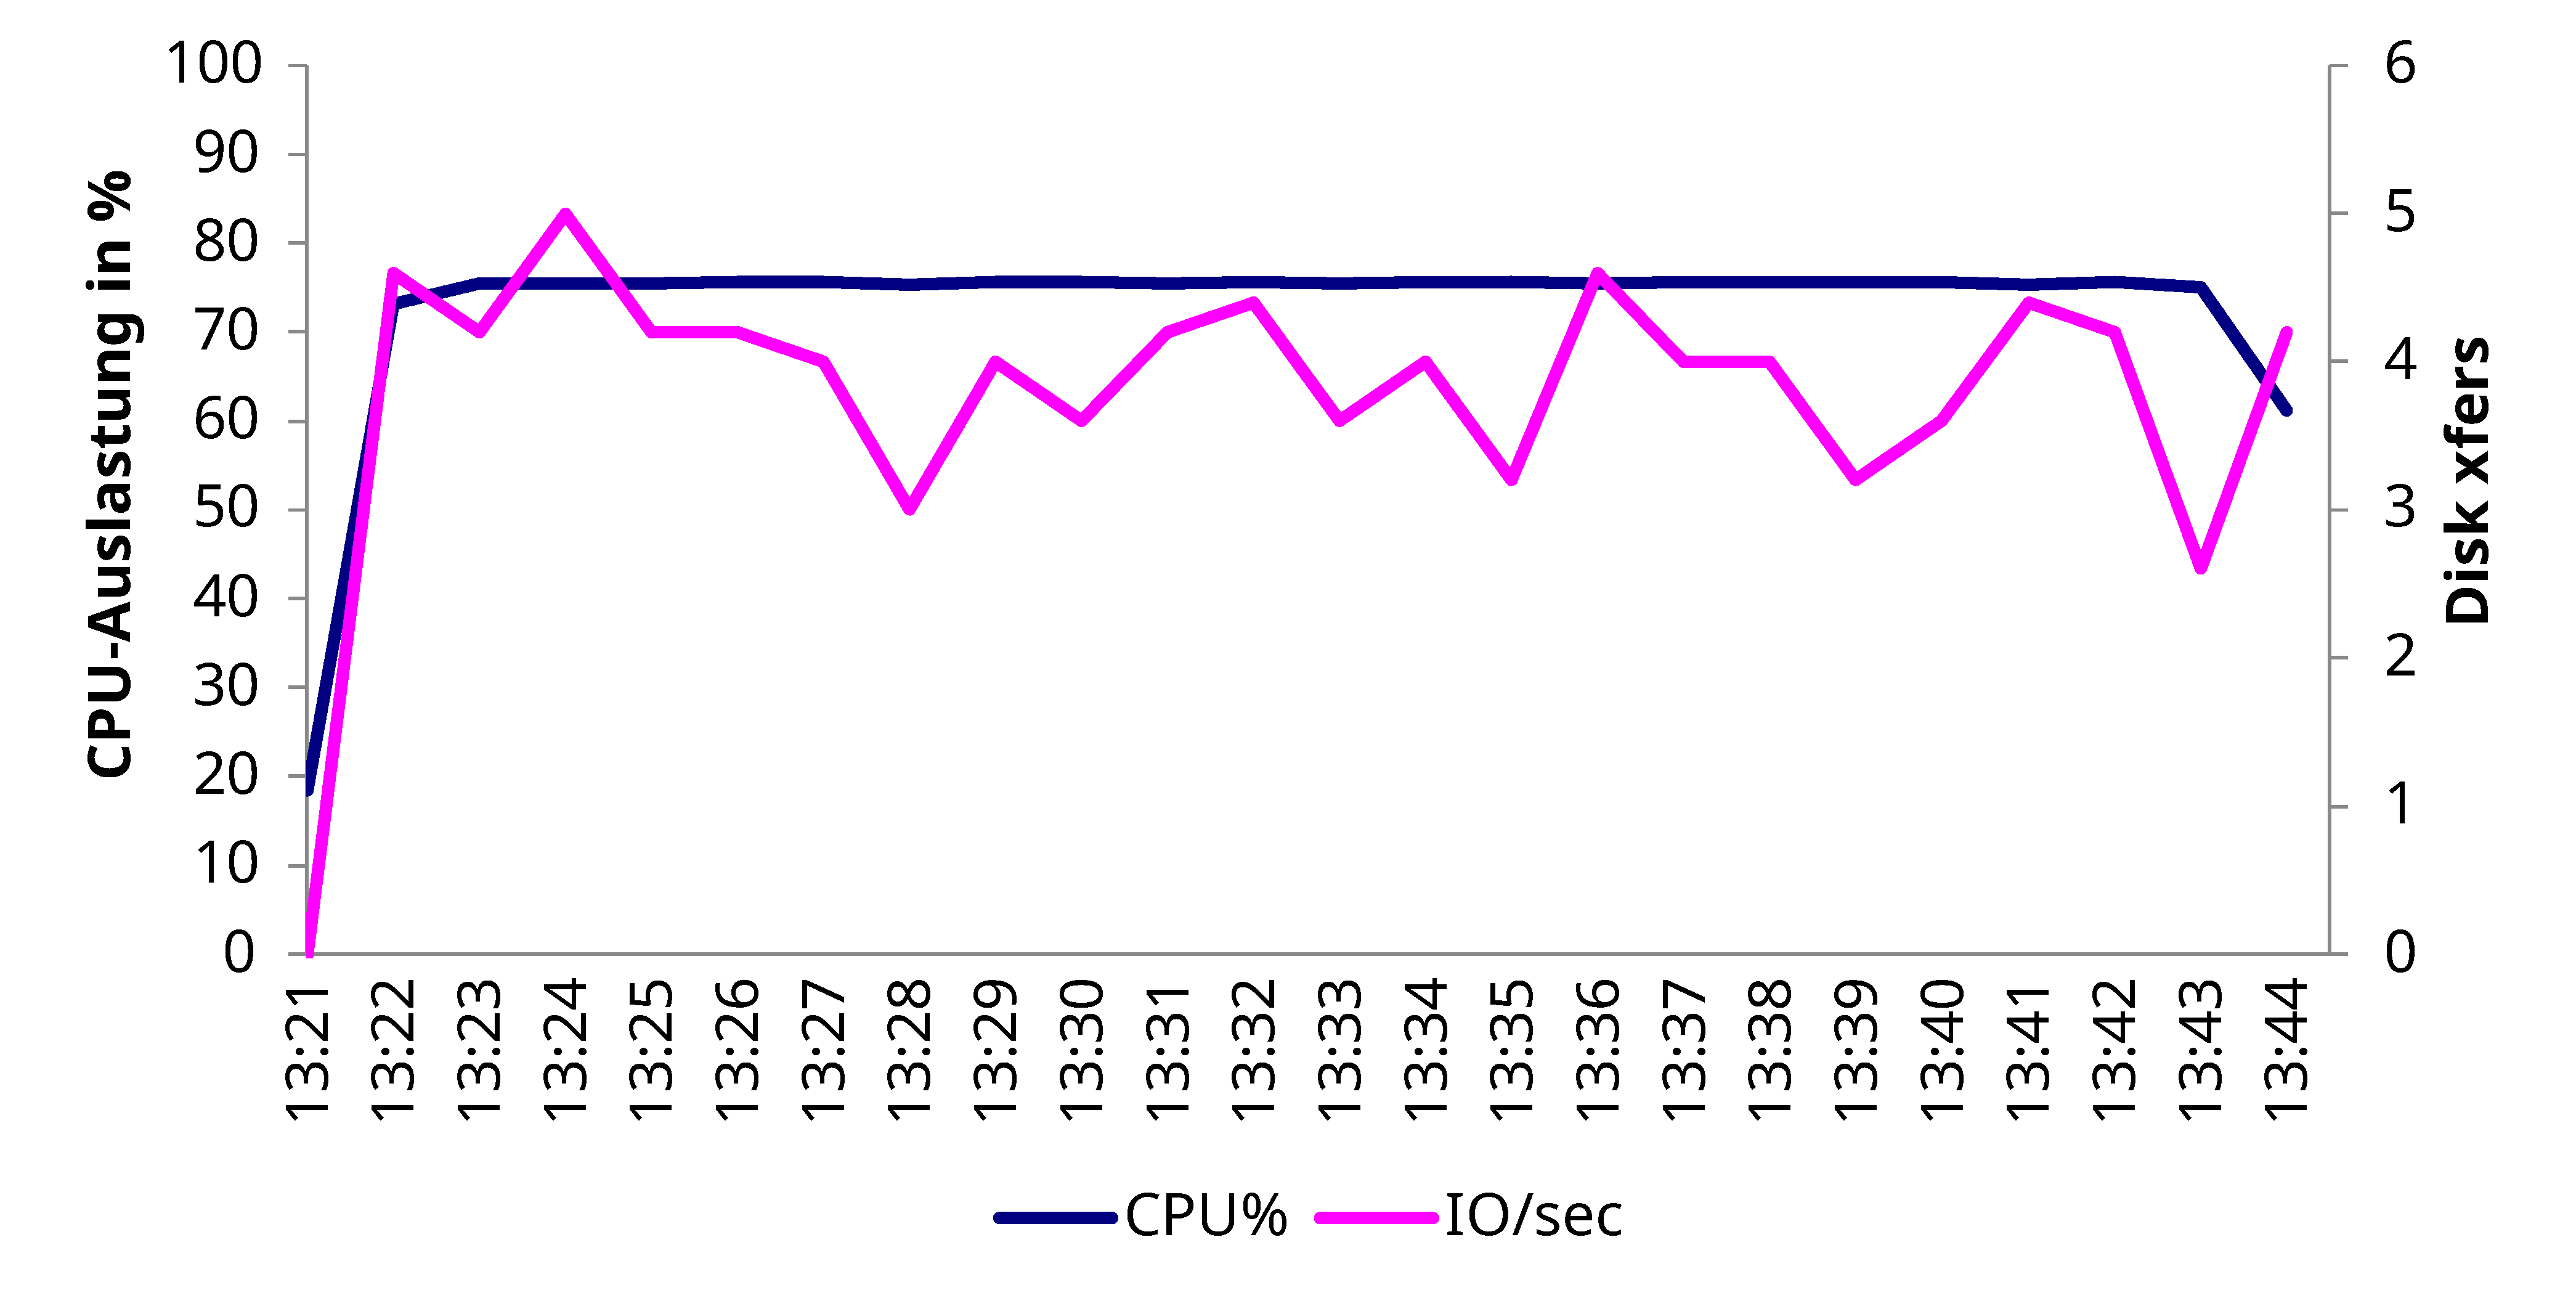
\includegraphics[width=\textwidth]{images/stats/linkbench-10m-const_neo4j.pdf}
    \caption{Linkbench-10M-Const Auslastung Neo4j (getNode)}
    \label{fig:nmon:10m:const:neo4j}
\end{figure}

\subsection{Linkbench-10M-Real}
\label{auswertung:ressourcenauslastung:real}
Bei den beiden im Rahmen dieser Messreihe aufgezeichneten Ressourcenstatistiken fällt bereits bei der ersten Begutachtung auf, dass die Statistiken für Db2 Graph V11.5.6.0 und besonders Neo4j über weitaus weniger Datenpunkte verfügen als die Abbildungen aus dem vorausgegangen \autoref{auswertung:ressourcenauslastung:const}. Dies ist dabei auf den Umstand zurückzuführen, dass die Messreihe, die auf Basis eines real-verteilten Datensatzes operieren, eine niedrigere Request-Anzahl pro Messung aufweisen als bei Messreihen mit konstanten-verteilten Datensätzen. Dies hat zur Folge, dass Neo4j und Db2 Graph V11.5.6.0 weniger Zeit für die Durchführung der Messungen benötigen. Der kleinere Messzeitraum sorgt dabei wiederum dafür, dass NMON weniger Datenpunkte für die Ressourcenstatistiken sammelt. Schließlich legt NMON während allen Messungen lediglich einen Datenpunkt pro Minute an. 

Bei der Analyse der CPU-Auslastung fällt auf, dass Neo4j \autoref{fig:nmon:10m:real:neo4j} und Db2 Graph V11.5.6.0 \autoref{fig:nmon:10m:real:ga} mit ca. durchschnittlich 76 \% und 39 \% ähnliche Werte wie im vorausgegangen \autoref{auswertung:ressourcenauslastung:const} darlegen. So verursacht Neo4j über seinen Messzeitraum eine höhere CPU-Auslastung als V11.5.6.0 bei seiner.   

Des Weiteren weisen beide Datenbanksysteme auch über den gesamten Verlauf der Messung ein Niveau auf, dass sie bis auf die erste Messung konstant halten. Wobei es hierbei zu beachten gilt, dass für diese Erhebung bei Neo4j lediglich vier Datenpunkte herangezogen werden.

Bei der IO-Auslastung hingegen kann bei Db2 Graph (\autoref{fig:nmon:10m:real:ga}) zu Beginn der Messung eine signifikante Spitze um 14:47 identifiziert werden. An diesem Punkt steigt die Anzahl an IO-Operationen (Disk xfers) kurzzeitig auf mehr als 7.000 pro Sekunde. Anschließend flacht die IO-Auslastung wieder auf die aus \autoref{auswertung:ressourcenauslastung:const} bekannten ca. 3.900 IO-Operationen pro Sekunde ab und hält diese bis zum Ende der Messung.

Die IO-Auslastung ist laut \autoref{fig:nmon:10m:real:neo4j} auch im Kontext dieser Messreihe mit im Maximalfall ca. 16 IO-Operationen pro Sekunde außergewöhnlich niedrig. Schließlich gilt es dabei zu beachten, dass auch die Read- und Write-Operationen auf den Festplattenspeicher von anderen Anwendung und System-Prozessen in der Statistik miterfasst werden. Die geringe IO-Auslastung bei Neo4j unterstützt dabei die in \autoref{auswertung:ressourcenauslastung:const} aufgestellte Hypothese, dass Neo4j scheinbar weitaus aggressiveres Caching als die Db2 Graph Versionen betreibt. 
\begin{figure}[!ht]
    \centering
    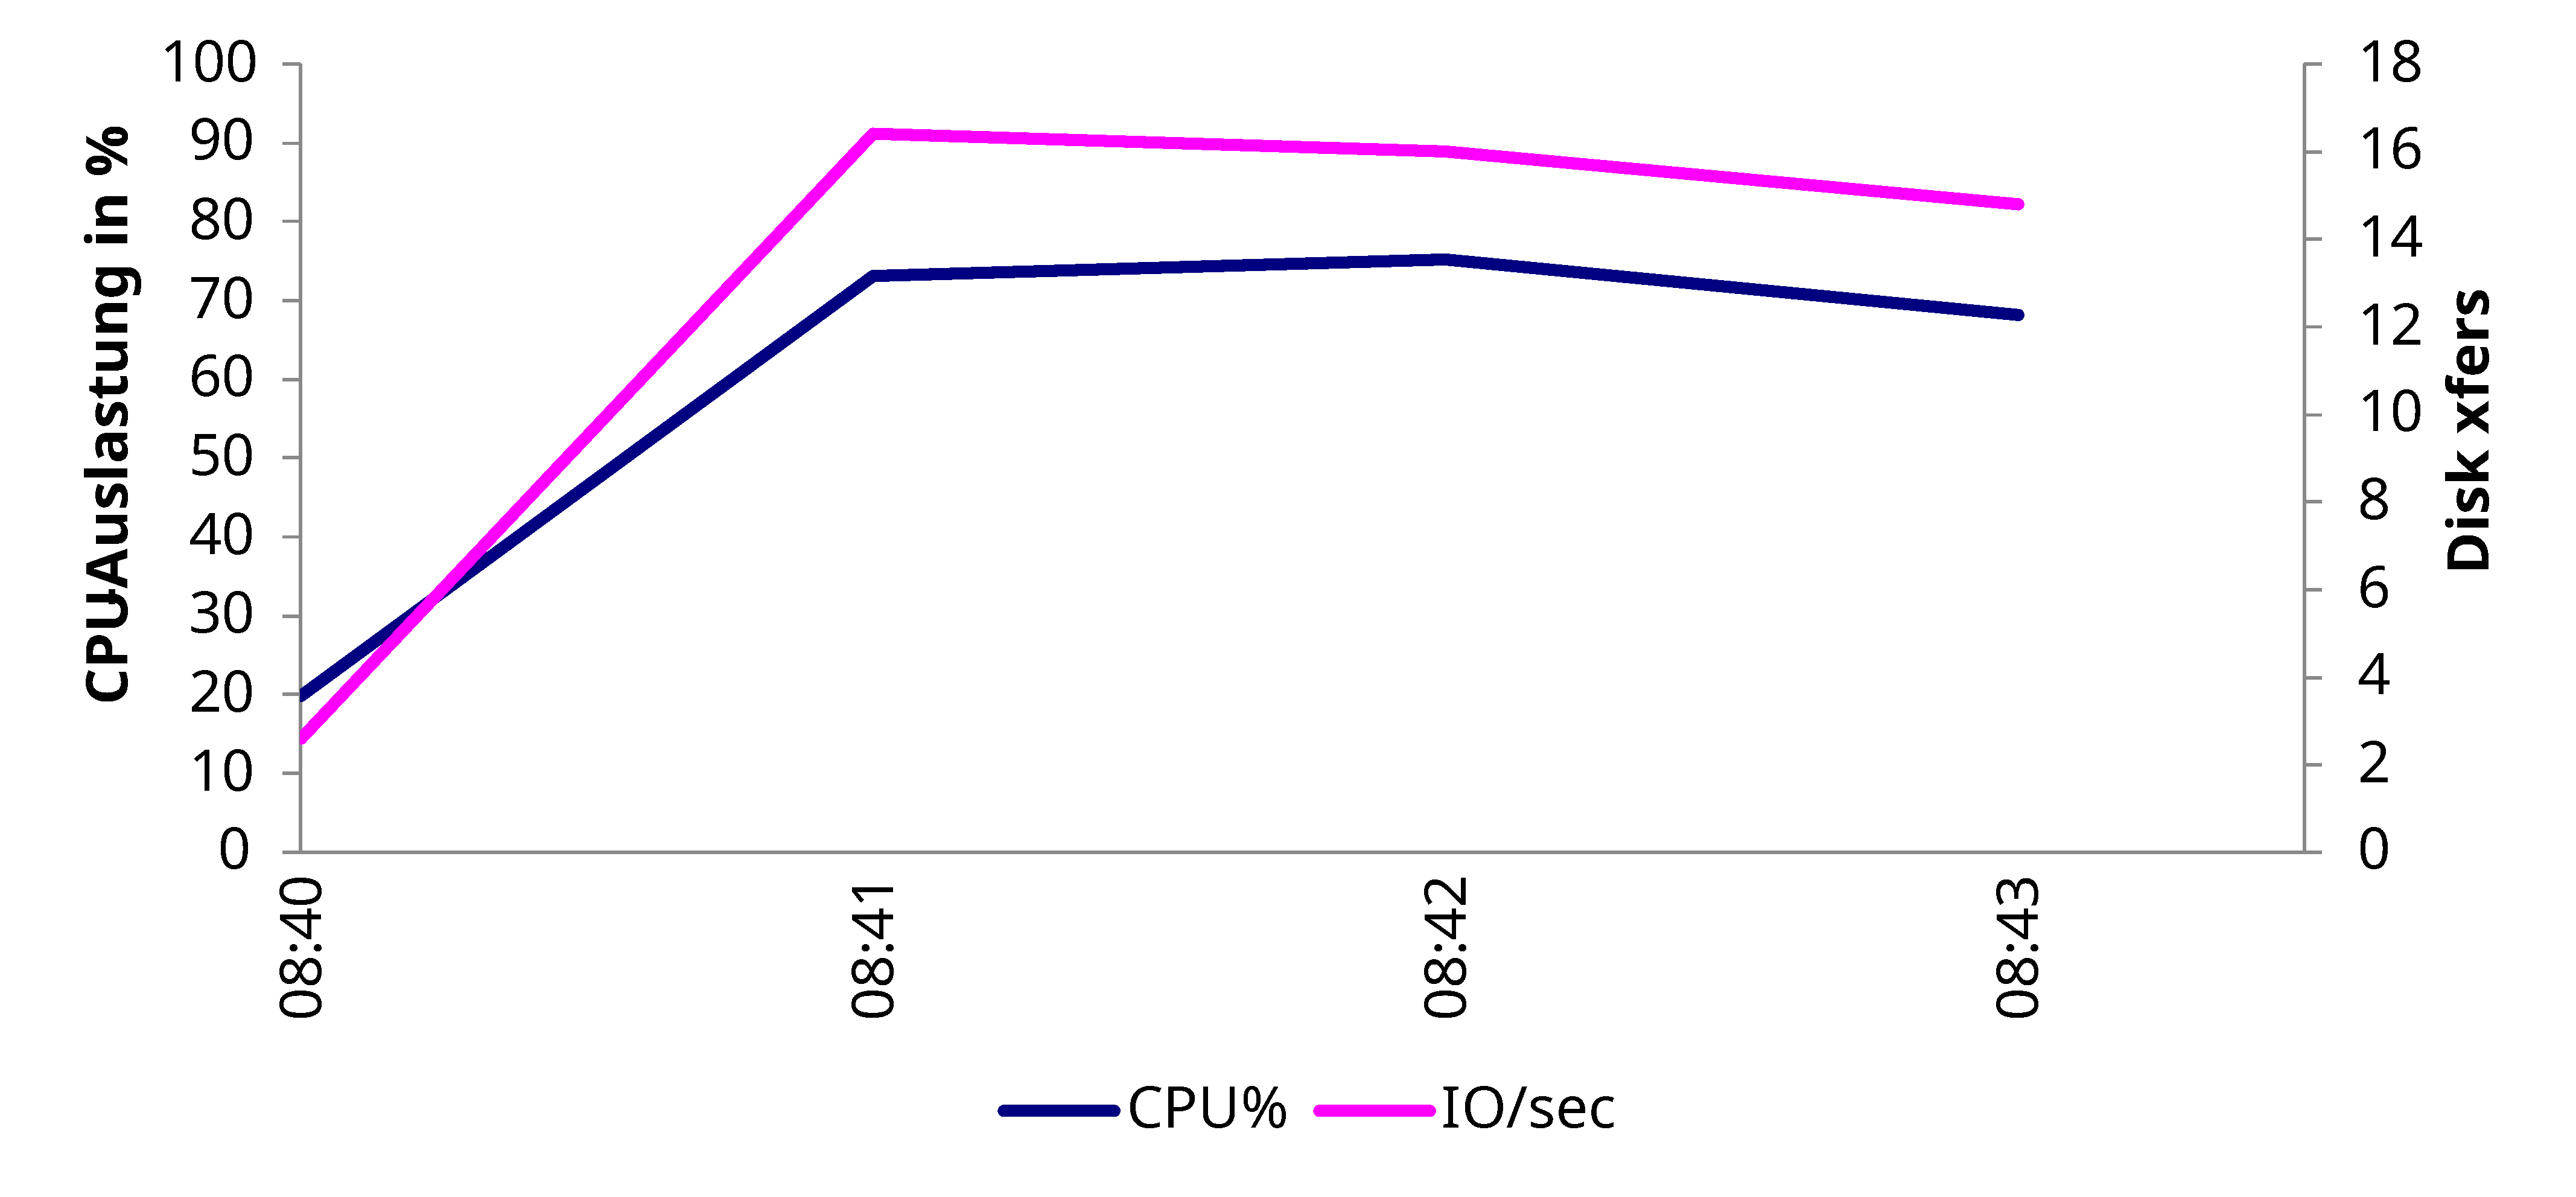
\includegraphics[width=\textwidth]{images/stats/linkbench-10m-real_ga.pdf}
    \caption{Linkbench-10M-Real Auslastung Db2 Graph V11.5.6.0 (getNode)}
    \label{fig:nmon:10m:real:ga}
\end{figure}

\begin{figure}[!ht]
    \centering
    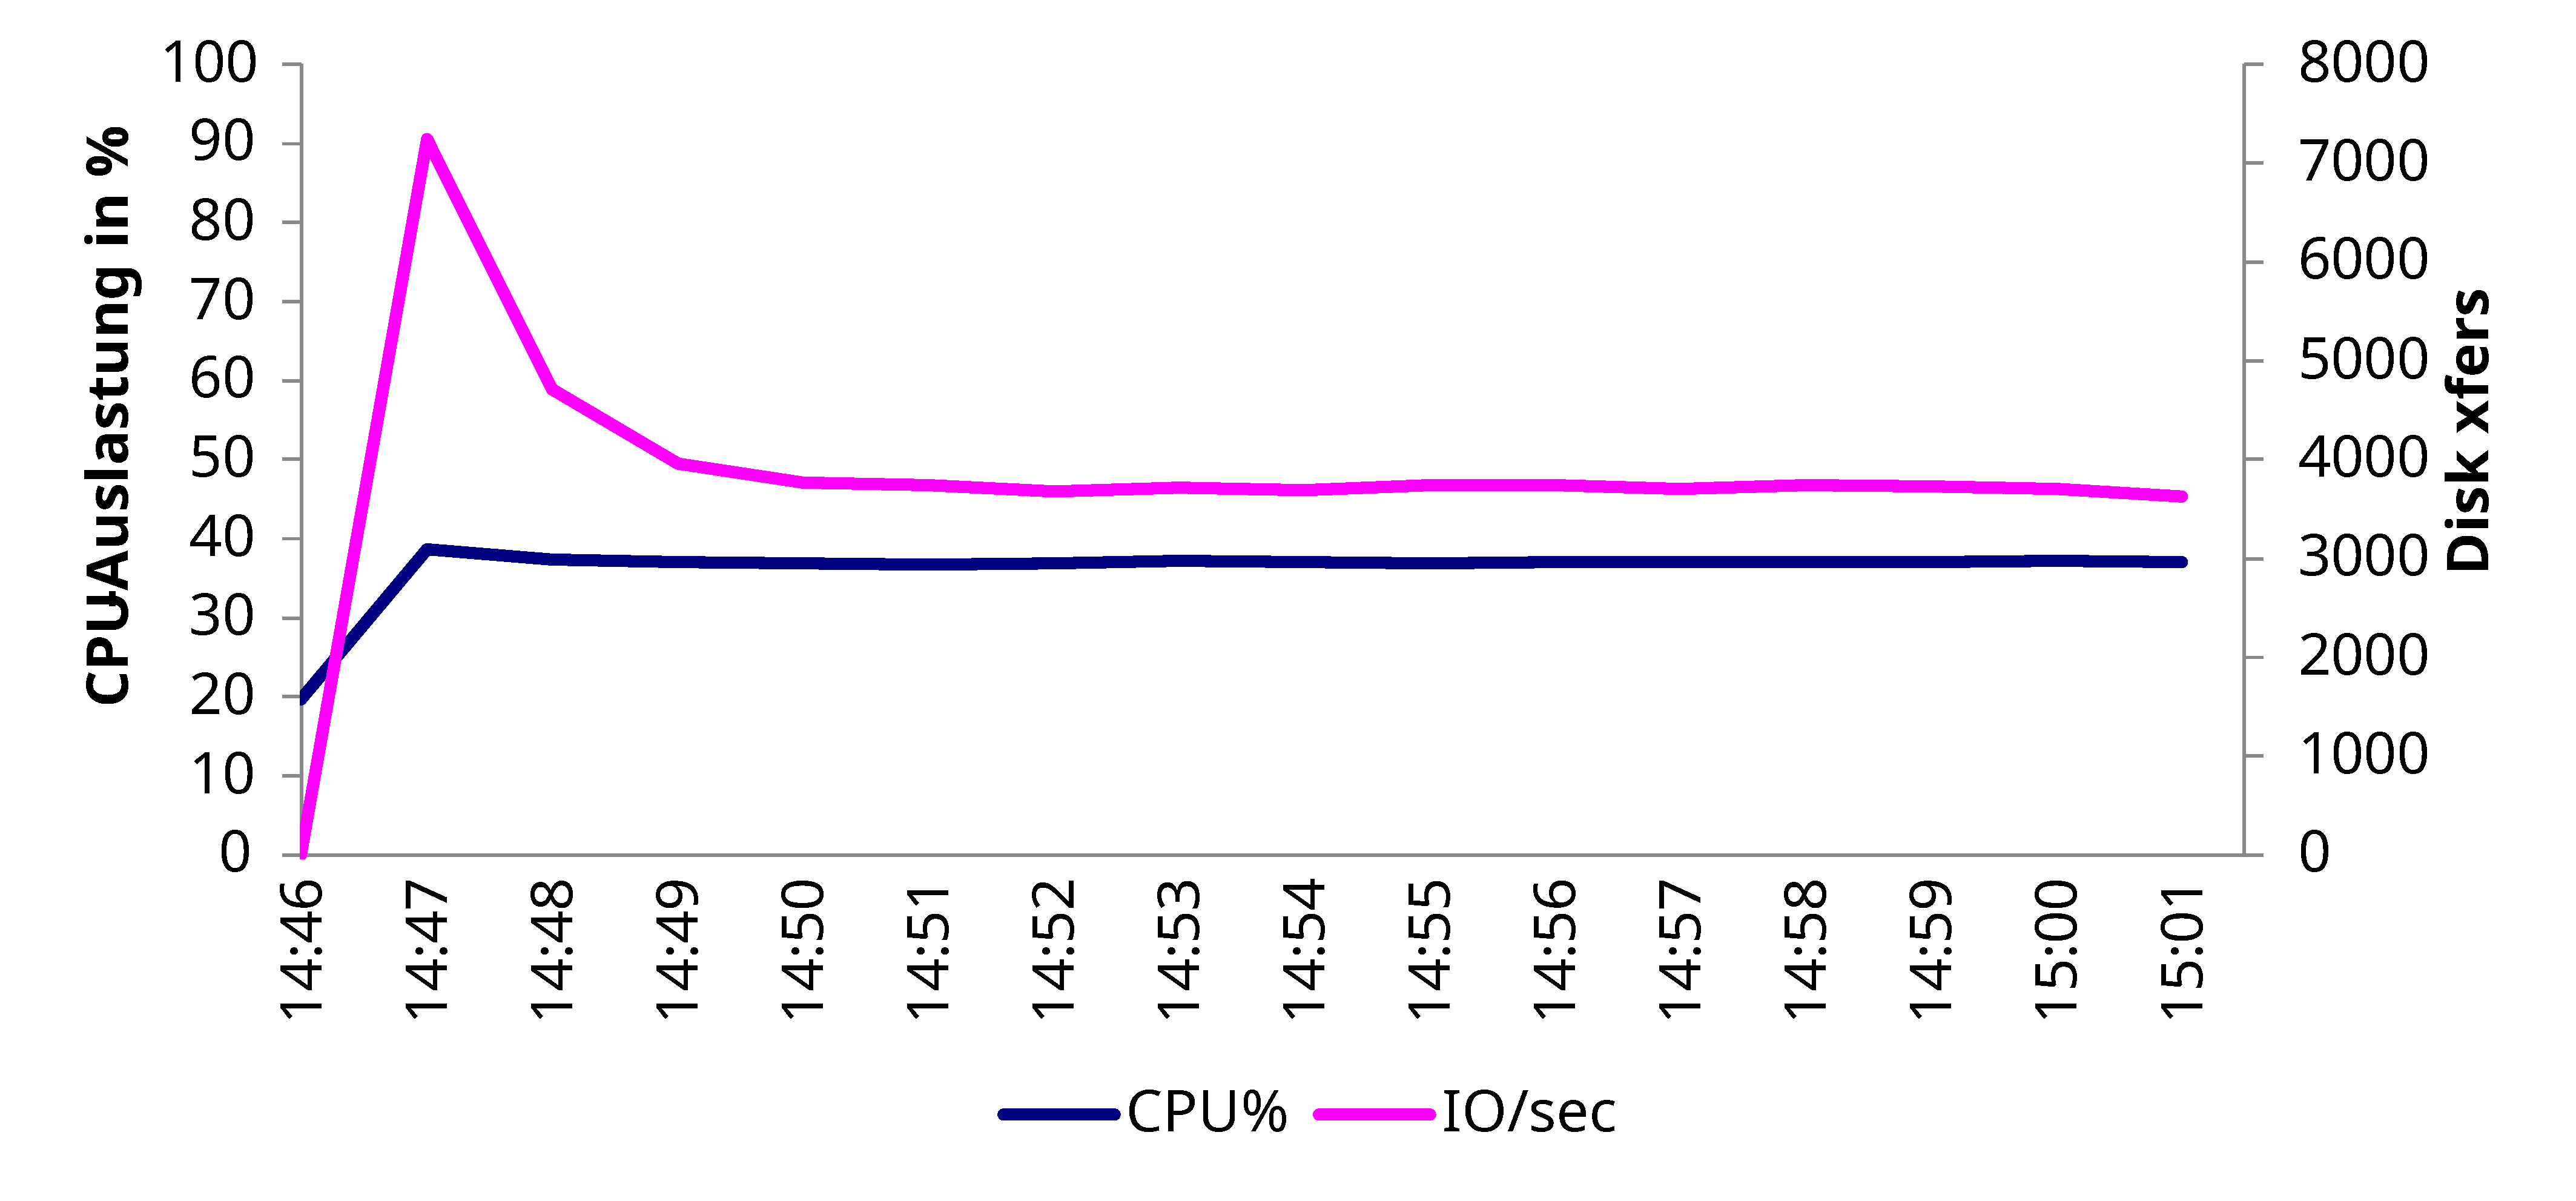
\includegraphics[width=\textwidth]{images/stats/linkbench-10m-real_neo4j.pdf}
    \caption{Linkbench-10M-Real Auslastung Neo4j (getNode)}
    \label{fig:nmon:10m:real:neo4j}
\end{figure}

\section{SQL-Anweisungen}
In diesem Abschnitt werden die von Db2 Graph Beta 3 und V11.5.6.0 generierten und an Db2 gesendeten SQL-Anweisungen miteinander verglichen und analysiert. Dieser Schritt wird hierbei durchgeführt, da der in \autoref{auswertung:einordnung} beschriebene signifikante Performance-Unterschied von Db2 Graph Beta 3 (der älteren weniger optimierten Version)  

\todo{Anhang einfügen}

\listoftodos